%\documentclass{article}
%\usepackage{beamerarticle}
\documentclass[serif,ignorenonframetext]{beamer}

% Macros for MATH 110 course dates

\newcommand{\commonTheme}{metropolis}
\newcommand{\commonColorTheme}{metropolis}

\newcommand{\commonAuthor}{Edward Doolittle}
\newcommand{\commonInstitute}{Department of Indigenous Knowledge and
  Science \\ First Nations University of Canada}
\newcommand{\commonCourse}{MATH 110 Calculus I}
\newcommand{\commonTerm}{202510}
\newcommand{\commonDate}{January 6, 2025}

% Review Material

% Lab 0
\newcommand{\commonEventNegativeOne}{LabNegativeOne}
\newcommand{\commonDateLabNegativeOne}{Monday, January 6, 2025}
\newcommand{\commonTitleLabNegativeOne}{MATH 110 Lab 0}
\newcommand{\commonSubtitleLabNegativeOne}{No Lab; Course Opens}

% Section 001
\newcommand{\commonEventZeroZeroOne}{ZeroZeroOne}
\newcommand{\commonDateZeroZeroOne}{Tuesday, January 7, 2025}
\newcommand{\commonTitleZeroZeroOne}{MATH 110 Review 0.1}
\newcommand{\commonSubtitleZeroZeroOne}{Review of Algebra}
\newcommand{\commonPSTitleZeroZeroOne}{MATH 110 Review Problem Set 0.1}

% Section 00A
\newcommand{\commonEventZeroZeroA}{ZeroZeroA}
\newcommand{\commonDateZeroZeroA}{Tuesday, January 7, 2025}
\newcommand{\commonTitleZeroZeroA}{MATH 110 Review 0.A}
\newcommand{\commonSubtitleZeroZeroA}{Review of Inequalities and
  Absolute Values}
\newcommand{\commonPSTitleZeroZeroA}{MATH 110 Review Problem Set 0.A}

% Section 00B
\newcommand{\commonEventZeroZeroB}{ZeroZeroB}
\newcommand{\commonDateZeroZeroB}{Tuesday, January 7, 2025}
\newcommand{\commonTitleZeroZeroB}{MATH 110 Review 0.B}
\newcommand{\commonSubtitleZeroZeroB}{Review of Coordinate Geometry
  and Lines}
\newcommand{\commonPSTitleZeroZeroB}{MATH 110 Review Problem Set 0.B}

% Section 00C
\newcommand{\commonEventZeroZeroC}{ZeroZeroC}
\newcommand{\commonDateZeroZeroC}{Thursday, January 9, 2025}
\newcommand{\commonTitleZeroZeroC}{MATH 110 Review 0.C}
\newcommand{\commonSubtitleZeroZeroC}{Review of Graphs of Second
  Degree Equations}
\newcommand{\commonPSTitleZeroZeroC}{MATH 110 Review Problem Set 0.C}

% Section 00D
\newcommand{\commonEventZeroZeroD}{ZeroZeroD}
\newcommand{\commonDateZeroZeroD}{Thursday, January 9, 2025}
\newcommand{\commonTitleZeroZeroD}{MATH 110 Review 0.D}
\newcommand{\commonSubtitleZeroZeroD}{Review of Trigonometry}
\newcommand{\commonPSTitleZeroZeroD}{MATH 110 Review Problem Set 0.D}

% Section 011
\newcommand{\commonEventZeroOneOne}{ZeroOneOne}
\newcommand{\commonDateZeroOneOne}{Thursday, January 9, 2025}
\newcommand{\commonTitleZeroOneOne}{MATH 110 Review 1.1}
\newcommand{\commonSubtitleZeroOneOne}{Review of Functions}
\newcommand{\commonPSTitleZeroOneOne}{MATH 110 Review Problem Set 1.1}


% Main Course

% Lab 1
\newcommand{\commonEventZero}{LabZero}
\newcommand{\commonDateLabZero}{Monday, January 13, 2025}
\newcommand{\commonTitleLabZero}{MATH 110 Lab 1}
\newcommand{\commonSubtitleLabZero}{Quiz 0: STACK, Onboarding}

% Section 1.4
\newcommand{\commonEventOne}{ZeroOneFour}
\newcommand{\commonDateZeroOneFour}{Tuesday, January 14, 2025}
\newcommand{\commonTitleZeroOneFour}{MATH 110 Lecture 1.4}
\newcommand{\commonSubtitleZeroOneFour}{The Tangent and Velocity Problems}
\newcommand{\commonPSTitleZeroOneFour}{MATH 110 Problem Set 1.4}

% Section 1.5
\newcommand{\commonEventTwo}{ZeroOneFive}
\newcommand{\commonDateZeroOneFive}{Thursday, January 16, 2025}
\newcommand{\commonTitleZeroOneFive}{MATH 110 Lecture 1.5}
\newcommand{\commonSubtitleZeroOneFive}{The Limit of a Function}
\newcommand{\commonPSTitleZeroOneFive}{MATH 110 Problem Set 1.5}

% Lab 2
\newcommand{\commonEventThree}{LabOne}
\newcommand{\commonDateLabOne}{Monday, January 20, 2025}
\newcommand{\commonTitleLabOne}{MATH 110 Lab 2}
\newcommand{\commonSubtitleLabOne}{Quiz 1: Review}

% Section 1.6
\newcommand{\commonEventFour}{ZeroOneSix}
\newcommand{\commonDateZeroOneSix}{Tuesday, January 21, 2025}
\newcommand{\commonTitleZeroOneSix}{MATH 110 Lecture 1.6}
\newcommand{\commonSubtitleZeroOneSix}{Calculating Limits Using the Limit Laws}
\newcommand{\commonPSTitleZeroOneSix}{MATH 110 Problem Set 1.6}

% Section 1.7
\newcommand{\commonEventFive}{ZeroOneSeven}
\newcommand{\commonDateZeroOneSeven}{(Not covered)}
\newcommand{\commonTitleZeroOneSeven}{MATH 110 Lecture 1.7}
\newcommand{\commonSubtitleZeroOneSeven}{The Precise Definition of a Limit}
\newcommand{\commonPSTitleZeroOneSeven}{MATH 110 Problem Set 1.7}

% Section 1.8
\newcommand{\commonEventSix}{ZeroOneEight}
\newcommand{\commonDateZeroOneEight}{Thursday, January 23, 2025}
\newcommand{\commonTitleZeroOneEight}{MATH 110 Lecture 1.8}
\newcommand{\commonSubtitleZeroOneEight}{Continuity}
\newcommand{\commonPSTitleZeroOneEight}{MATH 110 Problem Set 1.8}

% Lab 3
\newcommand{\commonEventSeven}{LabTwo}
\newcommand{\commonDateLabTwo}{Monday, January 27, 2025}
\newcommand{\commonTitleLabTwo}{MATH 110 Lab 3}
\newcommand{\commonSubtitleLabTwo}{Quiz 2: Sections 1.4, 1.5}

% Section 2.1
\newcommand{\commonEventEight}{ZeroTwoOne}
\newcommand{\commonDateZeroTwoOne}{Tuesday, January 28, 2025}
\newcommand{\commonTitleZeroTwoOne}{MATH 110 Lecture 2.1}
\newcommand{\commonSubtitleZeroTwoOne}{Derivatives and Rates of Change}
\newcommand{\commonPSTitleZeroTwoOne}{MATH 110 Problem Set 2.1}

% Section 2.2
\newcommand{\commonEventNine}{ZeroTwoTwo}
\newcommand{\commonDateZeroTwoTwo}{Thursday, January 30, 2025}
\newcommand{\commonTitleZeroTwoTwo}{MATH 110 Lecture 2.2}
\newcommand{\commonSubtitleZeroTwoTwo}{The Derivative as a Function}
\newcommand{\commonPSTitleZeroTwoTwo}{MATH 110 Problem Set 2.2}

% Lab 4
\newcommand{\commonEventTen}{LabThree}
\newcommand{\commonDateMTOne}{Monday, February 3, 2025} 
\newcommand{\commonDateLabThree}{Monday, February 3, 2025}
\newcommand{\commonTitleLabThree}{MATH 110 Lab 4}
\newcommand{\commonSubtitleLabThree}{Midterm: Review, Chapter 1}

% Section 2.3
\newcommand{\commonEventEleven}{ZeroTwoThree}
\newcommand{\commonDateZeroTwoThree}{Tuesday, February 4, 2025}
\newcommand{\commonTitleZeroTwoThree}{MATH 110 Lecture 2.3}
\newcommand{\commonSubtitleZeroTwoThree}{Differentiation Formulas}
\newcommand{\commonPSTitleZeroTwoThree}{MATH 110 Problem Set 2.3}

% Section 2.4
\newcommand{\commonEventTwelve}{ZeroTwoFour}
\newcommand{\commonDateZeroTwoFour}{Thursday, February 6, 2025}
\newcommand{\commonTitleZeroTwoFour}{MATH 110 Lecture 2.4}
\newcommand{\commonSubtitleZeroTwoFour}{Derivatives of Trigonometric Functions}
\newcommand{\commonPSTitleZeroTwoFour}{MATH 110 Problem Set 2.4}

% Lab 5
\newcommand{\commonEventThirteen}{LabFour}
\newcommand{\commonDateLabFour}{Monday, February 10, 2025}
\newcommand{\commonTitleLabFour}{MATH 110 Lab 5}
\newcommand{\commonSubtitleLabFour}{Quiz 3: Sections 2.1, 2.2}

% Section 2.5
\newcommand{\commonEventFourteen}{ZeroTwoFive}
\newcommand{\commonDateZeroTwoFive}{Tuesday, February 11, 2025}
\newcommand{\commonTitleZeroTwoFive}{MATH 110 Lecture 2.5}
\newcommand{\commonSubtitleZeroTwoFive}{The Chain Rule}
\newcommand{\commonPSTitleZeroTwoFive}{MATH 110 Problem Set 2.5}

% Section 2.6
\newcommand{\commonEventFifteen}{ZeroTwoSix}
\newcommand{\commonDateZeroTwoSix}{Thursday, February 13, 2025}
\newcommand{\commonTitleZeroTwoSix}{MATH 110 Lecture 2.6}
\newcommand{\commonSubtitleZeroTwoSix}{Implicit Differentiation}
\newcommand{\commonPSTitleZeroTwoSix}{MATH 110 Problem Set 2.6}

% Lab 6
\newcommand{\commonEventSixteen}{LabFive}
\newcommand{\commonDateLabFive}{Monday, February 24, 2025}
\newcommand{\commonTitleLabFive}{MATH 110 Lab 6}
\newcommand{\commonSubtitleLabFive}{Quiz 4: Sections 2.3, 2.4}

% Section 2.7
\newcommand{\commonEventSeventeen}{ZeroTwoSeven}
\newcommand{\commonDateZeroTwoSeven}{Tuesday, February 25, 2025}
\newcommand{\commonTitleZeroTwoSeven}{MATH 110 Lecture 2.7}
\newcommand{\commonSubtitleZeroTwoSeven}{Rates of Change in the
  Natural and Social Sciences}
\newcommand{\commonPSTitleZeroTwoSeven}{MATH 110 Problem Set 2.7}

% Section 2.8
\newcommand{\commonEventEighteen}{ZeroTwoEight}
\newcommand{\commonDateZeroTwoEight}{Thursday, February 27, 2025}
\newcommand{\commonTitleZeroTwoEight}{MATH 110 Lecture 2.8}
\newcommand{\commonSubtitleZeroTwoEight}{Related Rates}
\newcommand{\commonPSTitleZeroTwoEight}{MATH 110 Problem Set 2.8}

% Lab 7
\newcommand{\commonEventNineteen}{LabSix}
\newcommand{\commonDateLabSix}{Monday, March 3, 2025}
\newcommand{\commonTitleLabSix}{MATH 110 Lab 7}
\newcommand{\commonSubtitleLabSix}{Quiz 5: Sections 2.5, 2.6}

% Section 3.1
\newcommand{\commonEventTwenty}{ZeroThreeOne}
\newcommand{\commonDateZeroThreeOne}{Tuesday, March 4, 2025}
\newcommand{\commonTitleZeroThreeOne}{MATH 110 Lecture 3.1}
\newcommand{\commonSubtitleZeroThreeOne}{Maximum and Minimum Values}
\newcommand{\commonPSTitleZeroThreeOne}{MATH 11 Problem Set 3.1}

% Section 3.2
\newcommand{\commonEventTwentyOne}{ZeroThreeTwo}
\newcommand{\commonDateZeroThreeTwo}{Thursday, March 6, 2025}
\newcommand{\commonTitleZeroThreeTwo}{MATH 110 Lecture 3.2}
\newcommand{\commonSubtitleZeroThreeTwo}{The Mean Value Theorem}
\newcommand{\commonPSTitleZeroThreeTwo}{MATH 110 Problem Set 3.2}

% Lab 8
\newcommand{\commonEventTwentyTwo}{LabSeven}
\newcommand{\commonDateMTTwo}{Monday, March 10, 2025}
\newcommand{\commonDateLabSeven}{Monday, March 10, 2025}
\newcommand{\commonTitleLabSeven}{MATH 110 Lab 8}
\newcommand{\commonSubtitleLabSeven}{Midterm: Chapter 2}

% Section 3.3
\newcommand{\commonEventTwentyThree}{ZeroThreeThree}
\newcommand{\commonDateZeroThreeThree}{Tuesday, March 11, 2025}
\newcommand{\commonTitleZeroThreeThree}{MATH 110 Lecture 3.3}
\newcommand{\commonSubtitleZeroThreeThree}{How Derivatives Affect the
  Shape of a Graph}
\newcommand{\commonPSTitleZeroThreeThree}{MATH 110 Problem Set 3.3}

% Section 3.4
\newcommand{\commonEventTwentyFour}{ZeroThreeFour}
\newcommand{\commonDateZeroThreeFour}{Thursday, March 13, 2025}
\newcommand{\commonTitleZeroThreeFour}{MATH 110 Lecture 3.4}
\newcommand{\commonSubtitleZeroThreeFour}{Limits at Infinity;
  Horizontal Asymptotes}
\newcommand{\commonPSTitleZeroThreeFour}{MATH 110 Problem Set 3.4}

% Lab 9
\newcommand{\commonEventTwentyFive}{LabEight}
\newcommand{\commonDateLabEight}{Monday, March 17, 2025}
\newcommand{\commonTitleLabEight}{MATH 110 Lab 9}
\newcommand{\commonSubtitleLabEight}{Quiz 6: Sections 3.1, 3.2}

% Section 3.5
\newcommand{\commonEventTwentySix}{ZeroThreeFive}
\newcommand{\commonDateZeroThreeFive}{Tuesday, March 18, 2025}
\newcommand{\commonTitleZeroThreeFive}{MATH 110 Lecture 3.5}
\newcommand{\commonSubtitleZeroThreeFive}{Summary of Curve Sketching}
\newcommand{\commonPSTitleZeroThreeFive}{MATH 110 Problem Set 3.5}

% Section 3.7
\newcommand{\commonEventTwentySeven}{ZeroThreeSeven}
\newcommand{\commonDateZeroThreeSeven}{Thursday, March 20, 2025}
\newcommand{\commonTitleZeroThreeSeven}{MATH 110 Lecture 3.7}
\newcommand{\commonSubtitleZeroThreeSeven}{Optimization Problems}
\newcommand{\commonPSTitleZeroThreeSeven}{MATH 110 Problem Set 3.7}

% Lab 10
\newcommand{\commonEventTwentyEight}{LabNine}
\newcommand{\commonDateLabNine}{Monday, March 24, 2025}
\newcommand{\commonTitleLabNine}{MATH 110 Lab 10}
\newcommand{\commonSubtitleLabNine}{Quiz 7: Sections 3.3, 3.4}

% Section 4.1
\newcommand{\commonEventTwentyNine}{ZeroFourOne}
\newcommand{\commonDateZeroFourOne}{Tuesday, March 25, 2025}
\newcommand{\commonTitleZeroFourOne}{MATH 110 Lecture 4.1}
\newcommand{\commonSubtitleZeroFourOne}{Areas and Distances}
\newcommand{\commonPSTitleZeroFourOne}{MATH 110 Problem Set 4.1}

% Section 4.2
\newcommand{\commonEventThirty}{ZeroFourTwo}
\newcommand{\commonDateZeroFourTwo}{Thursday, March 27, 2025}
\newcommand{\commonTitleZeroFourTwo}{MATH 110 Lecture 4.2}
\newcommand{\commonSubtitleZeroFourTwo}{The Definite Integral}
\newcommand{\commonPSTitleZeroFourTwo}{MATH 110 Problem Set 4.2}

% Lab 11
\newcommand{\commonEventThirtyOne}{LabTen}
\newcommand{\commonDateLabTen}{Monday, March 31, 2025}
\newcommand{\commonTitleLabTen}{MATH 110 Lab 11}
\newcommand{\commonSubtitleLabTen}{Quiz 8: Sections 3.5, 3.7}

% Section 4.3
\newcommand{\commonEventThirtyTwo}{ZeroFourThree}
\newcommand{\commonDateZeroFourThree}{Tuesday, April 1, 2025}
\newcommand{\commonTitleZeroFourThree}{MATH 110 Lecture 4.3}
\newcommand{\commonSubtitleZeroFourThree}{The Fundamental Theorem of Calculus}
\newcommand{\commonPSTitleZeroFourThree}{MATH 110 Problem Set 4.3}

% Section 4.4
\newcommand{\commonEventThirtyThree}{ZeroFourFour}
\newcommand{\commonDateZeroFourFour}{Thursday, April 3, 2025}
\newcommand{\commonTitleZeroFourFour}{MATH 110 Lecture 4.4}
\newcommand{\commonSubtitleZeroFourFour}{Indefinite Integrals and the
  Net Change Theorem}
\newcommand{\commonPSTitleZeroFourFour}{MATH 110 Problem Set 4.4}

% Lab 12
\newcommand{\commonEventThirtyFour}{LabEleven}
\newcommand{\commonDateLabEleven}{Monday, April 7, 2025}
\newcommand{\commonTitleLabEleven}{MATH 110 Lab 12}
\newcommand{\commonSubtitleLabEleven}{Quiz 9: Sections 4.1, 4.2}

% Section 4.5
\newcommand{\commonEventThirtyFive}{ZeroFourFive}
\newcommand{\commonDateZeroFourFive}{Tuesday, April 8, 2025}
\newcommand{\commonTitleZeroFourFive}{MATH 110 Lecture 4.5}
\newcommand{\commonSubtitleZeroFourFive}{The Substitution Rule}
\newcommand{\commonPSTitleZeroFourFive}{MATH 110 Problem Set 4.5}

% Section 5.1
\newcommand{\commonEventThirtySix}{ZeroFiveOne}
\newcommand{\commonDateZeroFiveOne}{Thursday, April 10, 2025}
\newcommand{\commonTitleZeroFiveOne}{MATH 110 Lecture 5.1}
\newcommand{\commonSubtitleZeroFiveOne}{Areas Between Curves}
\newcommand{\commonPSTitleZeroFiveOne}{MATH 110 Problem Set 5.1}

% Lab 13
\newcommand{\commonEventThirtySeven}{LabTwelve}
\newcommand{\commonDateLabTwelve}{Monday, April 14, 2025}
\newcommand{\commonTitleLabTwelve}{MATH 110 Review Lab}
\newcommand{\commonSubtitleLabTwelve}{Bonus Quiz 10: Sections 4.3, 4.4}

% Final Class
\newcommand{\commonEventThirtyEight}{FinalClass}
\newcommand{\commonDateFinalClass}{Tuesday, April 15, 2025}
\newcommand{\commonTitleFinalClass}{MATH 110 Review Class}
\newcommand{\commonSubtitleFinalClass}{Answer Questions, Review for Exam}

% Final Exam
\newcommand{\commonEventThirtyNine}{Final}
\newcommand{\commonDateFinal}{Thursday, April 22, 2025}
\newcommand{\commonTitleFinal}{MATH 110 Final Exam}
\newcommand{\commonSubtitleFinal}{Comprehensive Exam: All Sections}

% Orphaned -- no longer part of the course

% Section 2.9
\newcommand{\commonDateZeroTwoNine}{Not part of the course}
\newcommand{\commonTitleZeroTwoNine}{MATH 110 Lecture 2.9}
\newcommand{\commonSubtitleZeroTwoNine}{Linear Approximations and Differentials}
\newcommand{\commonPSTitleZeroTwoNine}{MATH 110 Problem Set 2.9}


% % Introduction
% \newcommand{\commonEventOneDate}{Wednesday, September 8, 2010}
% \newcommand{\commonEventOneDesc}{Introduction to the Course}
% \newcommand{\commonDateZeroZeroZero}{September 8, 2010}
% \newcommand{\commonTitleZeroZeroZero}{MATH 104 Introduction}
% \newcommand{\commonSubtitleZeroZeroZero}{Outline of the Course}

% % Lecture 1
% \newcommand{\commonEventTwoDate}{Friday, September 10, 2010}
% \newcommand{\commonEventTwoDesc}{Lecture 1: Algebra}
% \newcommand{\commonDateZeroZeroOne}{September 10, 2010}
% \newcommand{\commonTitleZeroZeroOne}{MATH 104 Lecture 1}
% \newcommand{\commonSubtitleZeroZeroOne}{Review of Algebra}
% % associated evaluation ... factor this out?
% \newcommand{\commonPSTitleZeroZeroOne}{MATH 104 Problem Set 1}
% \newcommand{\commonEvalZeroZeroOne}{Quiz 1}
% \newcommand{\commonEvalDateZeroZeroOne}{Wednesday, September 15, 2010}

% % Lecture 2
% \newcommand{\commonEventThreeDate}{Monday, September 13, 2010}
% \newcommand{\commonEventThreeDesc}{Lecture 2: Appendix A}
% \newcommand{\commonDateZeroZeroA}{September 13, 2010}
% \newcommand{\commonTitleZeroZeroA}{MATH 104 Lecture 2}
% \newcommand{\commonSubtitleZeroZeroA}{Appendix A: Numbers, Inequalities, 
%   and Absolute Values}
% % associated evaluation ... factor this out?
% \newcommand{\commonPSTitleZeroZeroA}{MATH 104 Problem Set 2}
% \newcommand{\commonEvalZeroZeroA}{Quiz 2}
% \newcommand{\commonEvalDateZeroZeroA}{Wednesday, September 22, 2010}

% % Review 1
% \newcommand{\commonEventFourDate}{Wednesday, September 15, 2010}
% \newcommand{\commonEventFourDesc}{Review 1: Review Algebra; Quiz 1; Review Appendix A}
% \newcommand{\commonDateRZeroOne}{September 15, 2010}
% \newcommand{\commonTitleRZeroOne}{MATH 104 Review 1}
% \newcommand{\commonSubtitleRZeroOne}{Review of Algebra, Appendix A}

% % Lecture 3
% \newcommand{\commonEventFiveDate}{Friday, September 17, 2010}
% \newcommand{\commonEventFiveDesc}{Lecture 3: Appendix B}
% \newcommand{\commonDateZeroZeroB}{September 17, 2010}
% \newcommand{\commonTitleZeroZeroB}{MATH 104 Lecture 3}
% \newcommand{\commonSubtitleZeroZeroB}{Appendix B: Coordinate Geometry and Lines}
% % associated evaluation ... factor this out?
% \newcommand{\commonPSTitleZeroZeroB}{MATH 104 Problem Set 3}
% \newcommand{\commonEvalZeroZeroB}{Quiz 2}
% \newcommand{\commonEvalDateZeroZeroB}{Wednesday, September 22, 2010}

% % Lecture 4
% \newcommand{\commonEventSixDate}{Monday, Sepbember 20, 2010}
% \newcommand{\commonEventSixDesc}{Lecture 4: Appendix C}
% \newcommand{\commonDateZeroZeroC}{September 20, 2010}
% \newcommand{\commonTitleZeroZeroC}{MATH 104 Lecture 4}
% \newcommand{\commonSubtitleZeroZeroC}{Appendix C: Graphs of Second-Degree Equations}
% % associated evaluation ... factor this out?
% \newcommand{\commonPSTitleZeroZeroC}{MATH 104 Problem Set 4}
% \newcommand{\commonEvalZeroZeroC}{Midterm 0}
% \newcommand{\commonEvalDateZeroZeroC}{Wednesday, September 29, 2010}

% % Review 2
% \newcommand{\commonEventSevenDate}{Wednesday, September 22, 2010}
% \newcommand{\commonEventSevenDesc}{Review 2: Review Appendix B; Quiz 2; Review Appendix C}
% \newcommand{\commonDateRZeroTwo}{September 22, 2010}
% \newcommand{\commonTitleRZeroTwo}{MATH 104 Review 2}
% \newcommand{\commonSubtitleRZeroTwo}{Review of Appendices B and C}

% % Lecture 5
% \newcommand{\commonEventEightDate}{Friday, September 24, 2010}
% \newcommand{\commonEventEightDesc}{Lecture 5: Appendix D}
% \newcommand{\commonDateZeroZeroD}{September 24, 2010}
% \newcommand{\commonTitleZeroZeroD}{MATH 104 Lecture 5}
% \newcommand{\commonSubtitleZeroZeroD}{Appendix D: Trigonometry}
% % associated evaluation ... factor this out?
% \newcommand{\commonPSTitleZeroZeroD}{MATH 104 Problem Set 5}
% \newcommand{\commonEvalZeroZeroD}{Midterm 0}
% \newcommand{\commonEvalDateZeroZeroD}{Wednesday, September 29, 2010}

% % Lecture 6
% \newcommand{\commonEventNineDate}{Monday, September 27, 2010}
% \newcommand{\commonEventNineDesc}{Lecture 6: Section 1.1}
% \newcommand{\commonDateZeroOneOne}{September 27, 2010}
% \newcommand{\commonTitleZeroOneOne}{MATH 104 Lecture 6}
% \newcommand{\commonSubtitleZeroOneOne}{Section 1.1: Four Ways to Represent a Function}
% % associated evaluation ... factor this out?
% \newcommand{\commonPSTitleZeroOneOne}{MATH 104 Problem Set 6}
% \newcommand{\commonEvalZeroOneOne}{Quiz 3}
% \newcommand{\commonEvalDateZeroOneOne}{Wednesday, October 6, 2010}

% % Review 3
% \newcommand{\commonEventTenDate}{Wednesday, September 29, 2010}
% \newcommand{\commonEventTenDesc}{Review 3: Review Appendix D; 
%   Self-Assessment Midterm 0}
% \newcommand{\commonDateRZeroThree}{September 29, 2010}
% \newcommand{\commonTitleRZeroThree}{MATH 104 Review 3}
% \newcommand{\commonSubtitleRZeroThree}{Review of Appendix D}

% % Lecture 7
% \newcommand{\commonEventElevenDate}{Friday, October 1, 2010}
% \newcommand{\commonEventElevenDesc}{Lecture 7: Section 1.2}
% \newcommand{\commonDateZeroOneTwo}{October 1, 2010}
% \newcommand{\commonTitleZeroOneTwo}{MATH 104 Lecture 7}
% \newcommand{\commonSubtitleZeroOneTwo}{Section 1.2: Mathematical Models: A Catalog of Essential Functions}
% % associated evaluation ... factor this out?
% \newcommand{\commonPSTitleZeroOneTwo}{MATH 104 Problem Set 7}
% \newcommand{\commonEvalZeroOneTwo}{Quiz 3}
% \newcommand{\commonEvalDateZeroOneTwo}{Wednesday, October 6, 2010}

% % Lecture 8
% \newcommand{\commonEventTwelveDate}{Monday, October 4, 2010}
% \newcommand{\commonEventTwelveDesc}{Lecture 8: Section 1.3}
% \newcommand{\commonDateZeroOneThree}{October 4, 2010}
% \newcommand{\commonTitleZeroOneThree}{MATH 104 Lecture 8}
% \newcommand{\commonSubtitleZeroOneThree}{Section 1.3: New Functions from Old Functions}
% % associated evaluation ... factor this out?
% \newcommand{\commonPSTitleZeroOneThree}{MATH 104 Problem Set 8}
% \newcommand{\commonEvalZeroOneThree}{Quiz 4}
% \newcommand{\commonEvalDateZeroOneThree}{Wednesday, October 13, 2010}

% % Review 4
% \newcommand{\commonEventThirteenDate}{Wednesday, October 6, 2010}
% \newcommand{\commonEventThirteenDesc}{Review 4: Review 1.1, 1.2; Quiz 3}
% \newcommand{\commonDateROneOne}{October 6, 2010}
% \newcommand{\commonTitleROneOne}{MATH 104 Review 4}
% \newcommand{\commonSubtitleROneOne}{Reveiw of 1.1, 1.2}

% % Lecture 9
% \newcommand{\commonEventFourteenDate}{Friday, October 8, 2010}
% \newcommand{\commonEventFourteenDesc}{Lecture 9: Section 1.4}
% \newcommand{\commonDateZeroOneFour}{October 8, 2010}
% \newcommand{\commonTitleZeroOneFour}{MATH 104 Lecture 9}
% \newcommand{\commonSubtitleZeroOneFour}{Section 1.4: Graphing Calculators and Computers}
% % associated evaluation ... factor this out?
% \newcommand{\commonPSTitleZeroOneFour}{MATH 104 Problem Set 9}
% \newcommand{\commonEvalZeroOneFour}{Quiz 4}
% \newcommand{\commonEvalDateZeroOneFour}{Wednesday, October 13, 2010}

% % Thanksgiving holiday
% \newcommand{\commonEventFifteenDate}{Monday, October 11, 2010}
% \newcommand{\commonEventFifteenDesc}{No class: Thanksgiving holiday}

% % Review 5
% \newcommand{\commonEventSixteenDate}{Wednesday, October 13, 2010}
% \newcommand{\commonEventSixteenDesc}{Review 5: Review 1.3, 1.4; Quiz 4}
% \newcommand{\commonDateROneTwo}{October 13, 2010}
% \newcommand{\commonTitleROneTwo}{MATH 104 Review 5}
% \newcommand{\commonSubtitleOneRTwo}{Review of 1.3, 1.4}

% % Lecture 10
% \newcommand{\commonEventSeventeenDate}{Friday, October 15, 2010}
% \newcommand{\commonEventSeventeenDesc}{Lecture 10: Section 1.5}
% \newcommand{\commonDateZeroOneFive}{October 15, 2010}
% \newcommand{\commonTitleZeroOneFive}{MATH 104 Lecture 10}
% \newcommand{\commonSubtitleZeroOneFive}{Section 1.5: Exponential Functions}
% % associated evaluation ... factor this out?
% \newcommand{\commonPSTitleZeroOneFive}{MATH 104 Problem Set 10}
% \newcommand{\commonEvalZeroOneFive}{Quiz 5}
% \newcommand{\commonEvalDateZeroOneFive}{Wednesday, October 20, 2010}

% % Lecture 11
% \newcommand{\commonEventEighteenDate}{Monday, October 18, 2010}
% \newcommand{\commonEventEighteenDesc}{Lecture 11: Section 1.6}
% \newcommand{\commonDateZeroOneSix}{October 18, 2010}
% \newcommand{\commonTitleZeroOneSix}{MATH 104 Lecture 11}
% \newcommand{\commonSubtitleZeroOneSix}{Section 1.6: Inverse Functions and Logarithms}
% % associated evaluation ... factor this out?
% \newcommand{\commonPSTitleZeroOneSix}{MATH 104 Problem Set 11}
% \newcommand{\commonEvalZeroOneSix}{Midterm 1}
% \newcommand{\commonEvalDateZeroOneSix}{Wednesday, October 27, 2010}

% % Review 6
% \newcommand{\commonEventNineteenDate}{Wednesday, October 20, 2010}
% \newcommand{\commonEventNineteenDesc}{Review 6: Review 1.5; Quiz 5; Review 1.6}
% \newcommand{\commonDateROneThree}{October 20, 2010}
% \newcommand{\commonDateZeroOneR}{October 20, 2010}
% \newcommand{\commonTitleROneThree}{MATH 104 Review 6}
% \newcommand{\commonSubtitleROneThree}{Review of 1.5, 1.6}
% % associated evaluation ... factor this out?
% \newcommand{\commonPSTitleZeroOneR}{MATH 104 Problem Set R1}
% \newcommand{\commonEvalZeroOneR}{Midterm 1}
% \newcommand{\commonEvalDateZeroOneR}{Wednesday, October 27, 2010}

% % Lecture 12
% \newcommand{\commonEventTwentyDate}{Friday, October 22, 2010}
% \newcommand{\commonEventTwentyDesc}{Lecture 12: Section 2.1}
% \newcommand{\commonDateZeroTwoOne}{October 22, 2010}
% \newcommand{\commonTitleZeroTwoOne}{MATH 104 Lecture 12}
% \newcommand{\commonSubtitleZeroTwoOne}{Section 2.1: The Tangent and Velocity Problems}
% % associated evaluation ... factor this out?
% \newcommand{\commonPSTitleZeroTwoOne}{MATH 104 Problem Set 12}
% \newcommand{\commonEvalZeroTwoOne}{Quiz 6}
% \newcommand{\commonEvalDateZeroTwoOne}{Wednesday, November 3, 2010}

% % Lecture 13
% \newcommand{\commonEventTwentyOneDate}{Monday, October 25, 2010}
% \newcommand{\commonEventTwentyOneDesc}{Lecture 13: Section 2.2(a)}
% \newcommand{\commonDateZeroTwoTwoa}{October 25, 2010}
% \newcommand{\commonTitleZeroTwoTwoa}{MATH 104 Lecture 13}
% \newcommand{\commonSubtitleZeroTwoTwoa}{Section 2.2(a): The Limit of a Function I}
% % associated evaluation ... factor this out?
% \newcommand{\commonPSTitleZeroTwoTwoa}{MATH 104 Problem Set 13}
% \newcommand{\commonEvalZeroTwoTwoa}{Quiz 6}
% \newcommand{\commonEvalDateZeroTwoTwoa}{Wednesday, November 3, 2010}

% % Midterm Test 1
% % October 27, 2010
% \newcommand{\commonEventTwentyTwoDate}{Wednesday, October 27, 2010}
% \newcommand{\commonEventTwentyTwoDesc}{Midterm Test 1: Chapter 1}

% % Lecture 14
% \newcommand{\commonEventTwentyThreeDate}{Friday, October 29, 2010}
% \newcommand{\commonEventTwentyThreeDesc}{Lecture 14: Section 2.2(b)}
% \newcommand{\commonDateZeroTwoTwob}{October 29, 2010}
% \newcommand{\commonTitleZeroTwoTwob}{MATH 104 Lecture 14}
% \newcommand{\commonSubtitleZeroTwoTwob}{Section 2.2(b): The Limit of a Function II}
% % associated evaluation ... factor this out?
% \newcommand{\commonPSTitleZeroTwoTwob}{MATH 104 Problem Set 14}
% \newcommand{\commonEvalZeroTwoTwob}{Quiz 6}
% \newcommand{\commonEvalDateZeroTwoTwob}{Wednesday, November 3, 2010}

% % Lecture 15
% \newcommand{\commonEventTwentyFourDate}{Monday, November 1, 2010}
% \newcommand{\commonEventTwentyFourDesc}{Lecture 15: Section 2.3}
% \newcommand{\commonDateZeroTwoThree}{November 1, 2010}
% \newcommand{\commonTitleZeroTwoThree}{MATH 104 Lecture 15}
% \newcommand{\commonSubtitleZeroTwoThree}{Section 2.3: Calculating Limits Using the Limit Laws}
% % associated evaluation ... factor this out?
% \newcommand{\commonPSTitleZeroTwoThree}{MATH 104 Problem Set 15}
% \newcommand{\commonEvalZeroTwoThree}{Quiz 7}
% \newcommand{\commonEvalDateZeroTwoThree}{Wednesday, November 10, 2010}

% % Review 7
% \newcommand{\commonEventTwentyFiveDate}{Wednesday, November 3, 2010}
% \newcommand{\commonEventTwentyFiveDesc}{Review 7: Review 2.1, 2.2; Quiz 6; Review 2.3}
% \newcommand{\commonDateRTwoOne}{November 3, 2010}
% \newcommand{\commonTitleRTwoOne}{MATH 104 Review 7}
% \newcommand{\commonSubtitleRTwoOne}{Review of 2.1, 2.2, 2.3}

% % Lecture 16
% \newcommand{\commonEventTwentySixDate}{Friday, November 5, 2010}
% \newcommand{\commonEventTwentySixDesc}{Lecture 16: Section 2.5}
% \newcommand{\commonDateZeroTwoFive}{November 5, 2010}
% \newcommand{\commonTitleZeroTwoFive}{MATH 104 Lecture 16}
% \newcommand{\commonSubtitleZeroTwoFive}{Section 2.5: Continuity}
% % associated evaluation ... factor this out?
% \newcommand{\commonPSTitleZeroTwoFive}{MATH 104 Problem Set 16}
% \newcommand{\commonEvalZeroTwoFive}{Quiz 7}
% \newcommand{\commonEvalDateZeroTwoFive}{Wednesday, November 10, 2010}

% % Lecture 17
% \newcommand{\commonEventTwentySevenDate}{Monday, November 8, 2010}
% \newcommand{\commonEventTwentySevenDesc}{Lecture 17: Section 2.6}
% \newcommand{\commonDateZeroTwoSix}{November 8, 2010}
% \newcommand{\commonTitleZeroTwoSix}{MATH 104 Lecture 17}
% \newcommand{\commonSubtitleZeroTwoSix}{Section 2.6: Limits at Infinity: Horizontal Asymptotes}
% % associated evaluation ... factor this out?
% \newcommand{\commonPSTitleZeroTwoSix}{MATH 104 Problem Set 17}
% \newcommand{\commonEvalZeroTwoSix}{Quiz 8}
% \newcommand{\commonEvalDateZeroTwoSix}{Wednesday, November 17, 2010}

% % Review 8
% \newcommand{\commonEventTwentyEightDate}{Wednesday, November 10, 2010}
% \newcommand{\commonEventTwentyEightDesc}{Review 8: Review 2.5; Quiz 7; Review 2.6}
% \newcommand{\commonDateRTwoTwo}{November 10, 2010}
% \newcommand{\commonTitleRTwoTwo}{MATH 104 Review 8}
% \newcommand{\commonSubtitleRTwoTwo}{Review of 2.5, 2.6}

% % Lecture 18
% \newcommand{\commonEventTwentyNineDate}{Friday, November 12, 2010}
% \newcommand{\commonEventTwentyNineDesc}{Lecture 18: Section 2.7}
% \newcommand{\commonDateZeroTwoSeven}{November 12, 2010}
% \newcommand{\commonTitleZeroTwoSeven}{MATH 104 Lecture 18}
% \newcommand{\commonSubtitleZeroTwoSeven}{Section 2.7: Derivatives and Rates of Change}
% % associated evaluation ... factor this out?
% \newcommand{\commonPSTitleZeroTwoSeven}{MATH 104 Problem Set 18}
% \newcommand{\commonEvalZeroTwoSeven}{Quiz 8}
% \newcommand{\commonEvalDateZeroTwoSeven}{Wednesday, November 17, 2010}

% % Lecture 19
% \newcommand{\commonEventThirtyDate}{Monday, November 15, 2010}
% \newcommand{\commonEventThirtyDesc}{Lecture 19: Section 2.8}
% \newcommand{\commonDateZeroTwoEight}{November 15, 2010}
% \newcommand{\commonTitleZeroTwoEight}{MATH 104 Lecture 19}
% \newcommand{\commonSubtitleZeroTwoEight}{Section 2.8: The Derivative as a Function}
% % associated evaluation ... factor this out?
% \newcommand{\commonPSTitleZeroTwoEight}{MATH 104 Problem Set 19}
% \newcommand{\commonEvalZeroTwoEight}{Midterm 2}
% \newcommand{\commonEvalDateZeroTwoEight}{Wednesday, November 24, 2010}

% % Review 9
% % November 17, 2010
% \newcommand{\commonEventThirtyOneDate}{Wednesday, November 17, 2010}
% \newcommand{\commonEventThirtyOneDesc}{Review 9: Review 2.7; Quiz 8; Review 2.8}
% \newcommand{\commonDateRTwoThree}{November 17, 2010}
% \newcommand{\commonTitleRTwoThree}{MATH 104 Review 9}
% \newcommand{\commonSubtitleRTwoThree}{Review of 2.7, 2.8}

% % Lecture 20
% \newcommand{\commonEventThirtyTwoDate}{Friday, November 19, 2010}
% \newcommand{\commonEventThirtyTwoDesc}{Lecture 20: Section 3.1}
% \newcommand{\commonDateZeroThreeOne}{November 19, 2010}
% \newcommand{\commonTitleZeroThreeOne}{MATH 104 Lecture 20}
% \newcommand{\commonSubtitleZeroThreeOne}{Section 3.1: Derivatives of Polynomials and Exponential Functions}
% % associated evaluation ... factor this out?
% \newcommand{\commonPSTitleZeroThreeOne}{MATH 104 Problem Set 20}
% \newcommand{\commonEvalZeroThreeOne}{Quiz 9}
% \newcommand{\commonEvalDateZeroThreeOne}{Wednesday, December 1, 2010}

% % Lecture 21
% \newcommand{\commonEventThirtyThreeDate}{Monday, November 22, 2010}
% \newcommand{\commonEventThirtyThreeDesc}{Lecture 21: Section 3.2}
% \newcommand{\commonDateZeroThreeTwo}{November 22, 2010}
% \newcommand{\commonTitleZeroThreeTwo}{MATH 104 Lecture 21}
% \newcommand{\commonSubtitleZeroThreeTwo}{Section 3.2: The Product and Quotient Rules}
% % associated evaluation ... factor this out?
% \newcommand{\commonPSTitleZeroThreeTwo}{MATH 104 Problem Set 21}
% \newcommand{\commonEvalZeroThreeTwo}{Quiz 9}
% \newcommand{\commonEvalDateZeroThreeTwo}{Wednesday, December 1, 2010}

% % Midterm Test 2
% \newcommand{\commonEventThirtyFourDate}{Wednesday, November 24, 2010}
% \newcommand{\commonEventThirtyFourDesc}{Midterm Test 2: Chapter 2}

% % Lecture 22
% \newcommand{\commonEventThirtyFiveDate}{Friday, November 26, 2010}
% \newcommand{\commonEventThirtyFiveDesc}{Lecture 22: Section 3.3}
% \newcommand{\commonDateZeroThreeThree}{November 26, 2010}
% \newcommand{\commonTitleZeroThreeThree}{MATH 104 Lecture 22}
% \newcommand{\commonSubtitleZeroThreeThree}{Section 3.3: Derivatives of Trigonometric Functions}
% % associated evaluation ... factor this out?
% \newcommand{\commonPSTitleZeroThreeThree}{MATH 104 Problem Set 22}
% \newcommand{\commonEvalZeroThreeThree}{Quiz 9}
% \newcommand{\commonEvalDateZeroThreeThree}{Wednesday, December 1, 2010}

% % Lecture 23
% \newcommand{\commonEventThirtySixDate}{Monday, November 29, 2010}
% \newcommand{\commonEventThirtySixDesc}{Lecture 23: Section 3.4}
% \newcommand{\commonDateZeroThreeFour}{November 29, 2010}
% \newcommand{\commonTitleZeroThreeFour}{MATH 104 Lecture 23}
% \newcommand{\commonSubtitleZeroThreeFour}{Section 3.4: The Chain Rule}
% % associated evaluation ... factor this out?
% \newcommand{\commonPSTitleZeroThreeFour}{MATH 104 Problem Set 23}
% \newcommand{\commonEvalZeroThreeFour}{the final exam}
% \newcommand{\commonEvalDateZeroThreeFour}{Monday, December 13, 2010}

% % Review 10
% \newcommand{\commonEventThirtySevenDate}{Wednesday, December 1, 2010}
% \newcommand{\commonEventThirtySevenDesc}{Review 10: Review 3.1, 3.2, 3.3; Quiz 9}
% \newcommand{\commonDateRThreeTwo}{December 1, 2010}
% \newcommand{\commonTitleRThreeTwo}{MATH 104 Review 10}
% \newcommand{\commonSubtitleRThreeTwo}{Review of 3.1, 3.2, 3.3}

% % Lecture 24
% \newcommand{\commonEventThirtyEightDate}{Friday, December 3, 2010}
% \newcommand{\commonEventThirtyEightDesc}{Lecture 24: Section 3.5}
% \newcommand{\commonDateZeroThreeFive}{December 3, 2010}
% \newcommand{\commonTitleZeroThreeFive}{MATH 104 Lecture 24}
% \newcommand{\commonSubtitleZeroThreeFive}{Section 3.5: Implicit Differentiation}
% % associated evaluation ... factor this out?
% \newcommand{\commonPSTitleZeroThreeFive}{MATH 104 Problem Set 24}
% \newcommand{\commonEvalZeroThreeFive}{the final exam}
% \newcommand{\commonEvalDateZeroThreeFive}{Monday, December 13, 2010}

% % Lecture 25
% \newcommand{\commonEventThirtyNineDate}{Monday, December 6, 2010}
% \newcommand{\commonEventThirtyNineDesc}{Lecture 25: Section 3.6}
% \newcommand{\commonDateZeroThreeSix}{December 6, 2010}
% \newcommand{\commonTitleZeroThreeSix}{MATH 104 Lecture 25}
% \newcommand{\commonSubtitleZeroThreeSix}{Section 3.6: Derivatives of Logarithmic Functions}
% % associated evaluation ... factor this out?
% \newcommand{\commonPSTitleZeroThreeSix}{MATH 104 Problem Set 25}
% \newcommand{\commonEvalZeroThreeSix}{the final exam}
% \newcommand{\commonEvalDateZeroThreeSix}{Monday, December 13, 2010}

% % Review 11
% \newcommand{\commonEventFortyDate}{Wednesday, December 8, 2010}
% \newcommand{\commonEventFortyDesc}{(Bonus) Review 11: Review 3.4, 3.5, 3.6}
% \newcommand{\commonDateRThreeThree}{December 8, 2010}
% \newcommand{\commonTitleRThreeThree}{MATH 104 (Bonus) Review 11}
% \newcommand{\commonSubtitleRThreeThree}{Review of 3.4, 3.5, 3.6}

% % Final Exam
% % December 13, 2010
% \newcommand{\commonEventFinalDate}{Monday, December 13, 2010}
% \newcommand{\commonEventFinalDesc}{MATH 104 Final Exam}

%%% Local variables:
%%% mode: latex
%%% TeX-master: "MATH110-Syllabus.tex"
%%% End:

\usepackage{mathptmx}
\usepackage{multirow}
\usepackage{tikz}

\newcommand{\ds}{\displaystyle}

\mode<article>{}
\mode<presentation>{\usetheme{\commonTheme}\usecolortheme{\commonColorTheme}}

\title{\commonTitleZeroZeroD}
\subtitle{\commonSubtitleZeroZeroD}
\author{\commonAuthor}
\institute{\commonInstitute}
\date{\commonDateZeroZeroD}

\begin{document}

%\section*{Outline}

\begin{frame}
  \titlepage
\end{frame}

\begin{frame}
  \frametitle{Contents}
  \tableofcontents
\end{frame}


\section{Trigonometry}

% EJD: highlight final answers in formulas!

\subsection{Angles}

\begin{frame}
  \frametitle{Radian Measure}
  \begin{columns}
  \column{0.65\textwidth}
  \begin{itemize}[<+->]
  \item The system of degrees we often use to measure angles is based
    on an arbitrary choice of $360^{\circ}$ for a whole circle.
  \item It is better to use a more natural measure for angles,
    \textit{radians}. 
  \item One radian is the angle subtended by a length of one radius
    marked out around the circle.
  \item The circumference of a circle is $2\pi r$, so a full circle is
    $2\pi$ radians.
  \end{itemize}
  \column{0.35\textwidth}
  \only<1-2>{ %
    \begin{tikzpicture}[scale=0.29]
      \draw (0,0) circle (6);
    \end{tikzpicture}
  }
  \only<3>{ %
    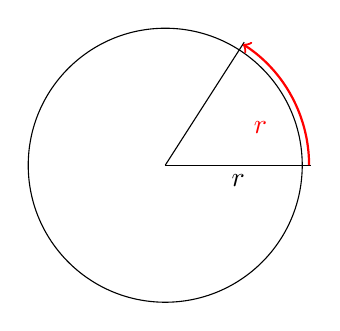
\begin{tikzpicture}[scale=0.29]
      \draw (0,0) circle (6);
      \draw (0,0) -- node[midway,below]{$r$} (6.4,0);
      \draw (0,0) -- (57.30:6.4);
      \draw[red,thick,->] (6.3,0) arc (0:57.30:6.3);
      \draw[red] node[label={225:$r$}] (A) at (27.65:6) {};
    \end{tikzpicture}
  }
  \only<4>{ %
    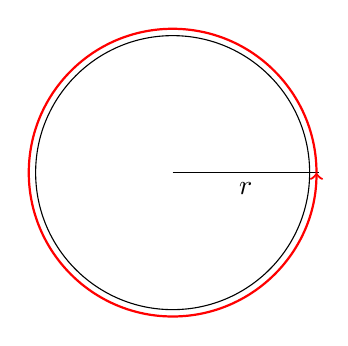
\begin{tikzpicture}[scale=0.29]
      \draw (0,0) circle (6);
      \draw (0,0) -- node[midway,below]{$r$} (6.4,0);
      \draw[red,thick,->] (6.3,0) arc (0:360:6.3);
    \end{tikzpicture}
  }
  \end{columns}
\end{frame}

\begin{frame}
  \frametitle{Common Conversions}
  \begin{columns}
  \column{0.65\textwidth}
  \begin{itemize}[<+->]
  \item A full circle is $360^{\circ}$ which is $2\pi$ radians.
  \item Half a circle is $180^{\circ}$ which is $\pi$ radians.
  \item A quarter circle is $90^{\circ}$ which is $\pi/2$ radians.
  \item An eighth of a circle is $45^{\circ}$ which is $\pi/4$
    radians.
  \item A sixth of a circle is $60^{\circ}$ which is $2\pi/6=\pi/3$
    radians.
  \item A twelfth of a circle is $30^{\circ}$ which is $2\pi/12=\pi/6$
    radians. 
  \end{itemize}
  \column{0.35\textwidth}
  \only<1>{ %
    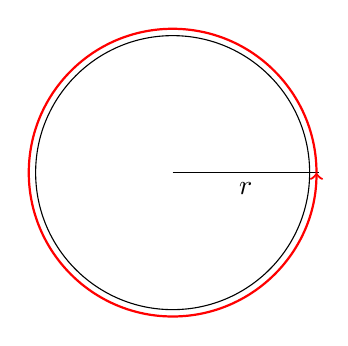
\begin{tikzpicture}[scale=0.29]
      \draw (0,0) circle (6);
      \draw (0,0) -- node[midway,below]{$r$} (6.4,0);
      \draw[red,thick,->] (6.3,0) arc (0:360:6.3);
    \end{tikzpicture}
  }
  \only<2>{ %
    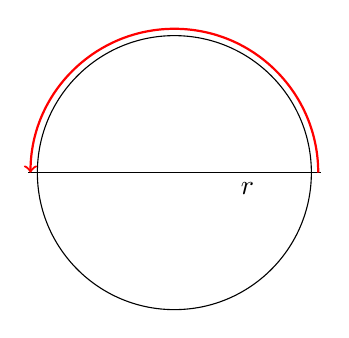
\begin{tikzpicture}[scale=0.29]
      \draw (0,0) circle (6);
      \draw (0,0) -- node[midway,below]{$r$} (6.4,0);
      \draw (0,0) -- (180:6.4);
      \draw[red,thick,->] (6.3,0) arc (0:180:6.3);
    \end{tikzpicture}
  }
  \only<3>{ %
    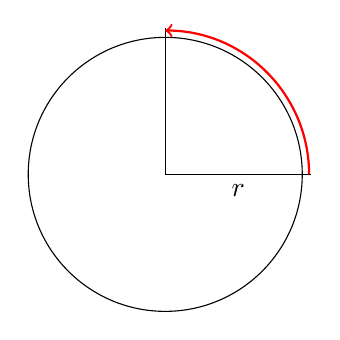
\begin{tikzpicture}[scale=0.29]
      \draw (0,0) circle (6);
      \draw (0,0) -- node[midway,below]{$r$} (6.4,0);
      \draw (0,0) -- (90:6.4);
      \draw[red,thick,->] (6.3,0) arc (0:90:6.3);
    \end{tikzpicture}
  }
  \only<4>{ %
    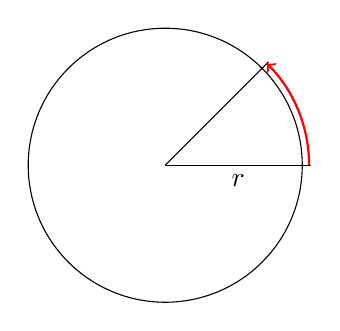
\begin{tikzpicture}[scale=0.29]
      \draw (0,0) circle (6);
      \draw (0,0) -- node[midway,below]{$r$} (6.4,0);
      \draw (0,0) -- (45:6.4);
      \draw[red,thick,->] (6.3,0) arc (0:45:6.3);
    \end{tikzpicture}
  }
  \only<5>{ %
    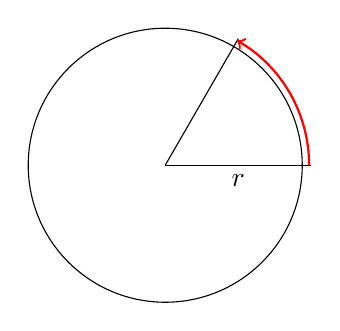
\begin{tikzpicture}[scale=0.29]
      \draw (0,0) circle (6);
      \draw (0,0) -- node[midway,below]{$r$} (6.4,0);
      \draw (0,0) -- (60:6.4);
      \draw[red,thick,->] (6.3,0) arc (0:60:6.3);
    \end{tikzpicture}
  }
  \only<6>{ %
    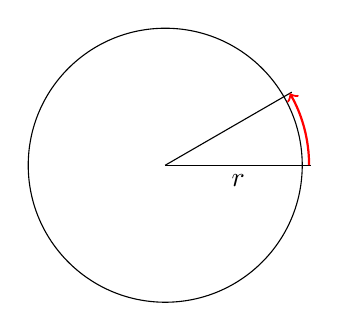
\begin{tikzpicture}[scale=0.29]
      \draw (0,0) circle (6);
      \draw (0,0) -- node[midway,below]{$r$} (6.4,0);
      \draw (0,0) -- (30:6.4);
      \draw[red,thick,->] (6.3,0) arc (0:30:6.3);
    \end{tikzpicture}
  }
  \end{columns}
\end{frame}

% EJD: diagrams of circular arc
\begin{frame}
  \frametitle{Length of a Circular Arc}
  \begin{columns}
  \column{0.65\textwidth}
  \begin{itemize}[<+->]
  \item Similar proportional reasoning applies to the length of a
    circular arc.
  \item The arc length of a whole circle is $2\pi r$, the angle in
    radians times the radius.
  \item The arc length of half a circle is $\pi r$, the angle in
    radians times the radius.
  \item The arc length of a quarter circle is $(\pi/2)r$, the angle in
    radians times the radius.
  \item In general, the arc length of any arc is the angle subtended
    by the arc in radians times the radius.
  \end{itemize}
  \column{0.35\textwidth}
  \only<1-2>{ %
    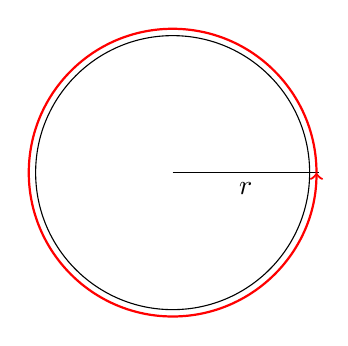
\begin{tikzpicture}[scale=0.29]
      \draw (0,0) circle (6);
      \draw (0,0) -- node[midway,below]{$r$} (6.4,0);
      \draw[red,thick,->] (6.3,0) arc (0:360:6.3);
    \end{tikzpicture}
  }
  \only<3>{ %
    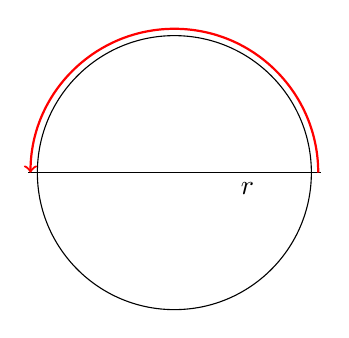
\begin{tikzpicture}[scale=0.29]
      \draw (0,0) circle (6);
      \draw (0,0) -- node[midway,below]{$r$} (6.4,0);
      \draw (0,0) -- (180:6.4);
      \draw[red,thick,->] (6.3,0) arc (0:180:6.3);
    \end{tikzpicture}
  }
  \only<4>{ %
    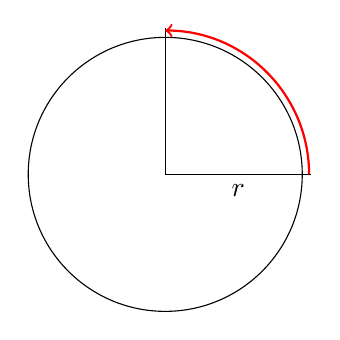
\begin{tikzpicture}[scale=0.29]
      \draw (0,0) circle (6);
      \draw (0,0) -- node[midway,below]{$r$} (6.4,0);
      \draw (0,0) -- (90:6.4);
      \draw[red,thick,->] (6.3,0) arc (0:90:6.3);
    \end{tikzpicture}
  }
  \only<5>{ %
    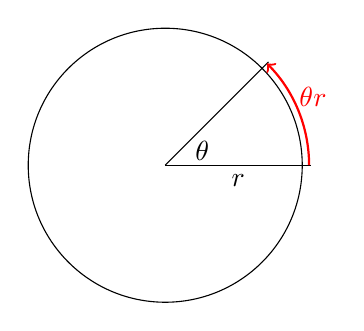
\begin{tikzpicture}[scale=0.29]
      \draw (0,0) circle (6);
      \draw (0,0) -- node[midway,below]{$r$} (6.4,0);
      \draw (0,0) -- (45:6.4);
      \draw node[label={$\theta$}] at (-22.5:1.75) {};
      \draw[red,thick,->] (6.3,0) arc (0:45:6.3) ;
      \draw[red] node[label={$\theta r$}] (A) at (15:6.7) {};
    \end{tikzpicture}
  }
  \end{columns}
\end{frame}

%% \begin{frame}
%%   \frametitle{The Meaning of the Radian}
%%   \begin{columns}
%%   \column{0.65\textwidth}
%%   \begin{itemize}[<+->]
%%   \item 1
%%   \item 2
%%   \end{itemize}
%%   \column{0.35\textwidth}
%%   \end{columns}
%% \end{frame}

% EJD: blow-up of unit circle
\begin{frame}
  \frametitle{Angles in Standard Position}
  \begin{columns}
  \column{0.65\textwidth}
  \begin{itemize}[<+->]
  \item We often work with a particular circle, the unit circle on the
    Cartesian plane.
  \item In that context, we measure angles from the $x$-axis
    counter-clockwise. 
  \item Angles from $0$ to $\pi/2$ radians are said to be in the first
    quadrant. 
  \item Angles from $\pi/2$ to $\pi$ radians are said to be in the
    second quadrant.
  \end{itemize}
  \column{0.35\textwidth}
  \only<1>{ %
    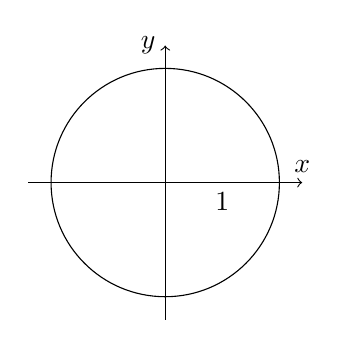
\begin{tikzpicture}[scale=0.29]
      \draw (0,0) circle (5);
      \draw[->] (-6,0) -- (0,0) -- node[midway,below]{$1$} (5,0) -- (6,0) node[above]{$x$};
      \draw[->] (0,-6) -- (0,6) node[left]{$y$};
    \end{tikzpicture}
  }
  \only<2-3>{ %
    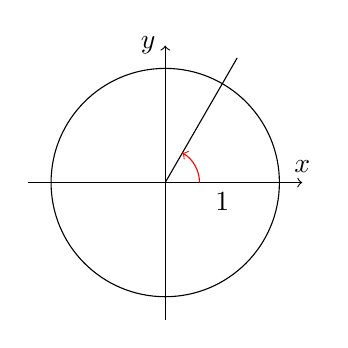
\begin{tikzpicture}[scale=0.29]
      \draw (0,0) circle (5);
      \draw[->] (-6,0) -- (0,0) -- node[midway,below]{$1$} (5,0) -- (6,0) node[above]{$x$};
      \draw[->] (0,-6) -- (0,6) node[left]{$y$};
      \draw (0,0) -- (60:6.3);
      \draw[red,->] (1.5,0) arc (0:60:1.5);
    \end{tikzpicture}
  }
  \only<4>{ %
    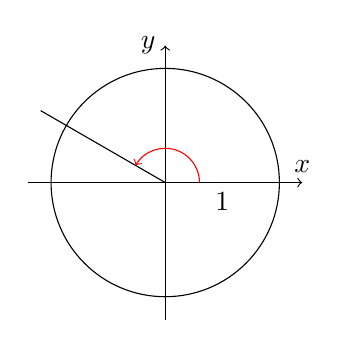
\begin{tikzpicture}[scale=0.29]
      \draw (0,0) circle (5);
      \draw[->] (-6,0) -- (0,0) -- node[midway,below]{$1$} (5,0) -- (6,0) node[above]{$x$};
      \draw[->] (0,-6) -- (0,6) node[left]{$y$};
      \draw (0,0) -- (150:6.3);
      \draw[red,->] (1.5,0) arc (0:150:1.5);
    \end{tikzpicture}
  }
  \end{columns}
\end{frame}


\subsection{The Trigonometric Functions}

% EJD: might be best to use unit circles for everything,
% so don't use 1,1,\sqrt[2} triangle but 1/\sqrt{2}, 1/\sqrt{2}, 1 triangle

\begin{frame}
  \frametitle{Right Triangles}
  \begin{columns}
  \column{0.65\textwidth}
  \begin{itemize}[<+->]
  \item<1-> The easiest way to explore angles is to use right triangles.
  \item<2-> We orient the base of the triangle horizontally, with the
    right angle (usually) on the right.
  \item<3-> The longest side is called the \textit{hypoteneuse}.  The
    other sides are called \textit{legs}.
  \item<4-> We focus on the non-right angle on the base, we call that
    \textit{the angle}.
  \item<5-> The leg between the angle and the right angle is called
    \textit{adjacent}.
  \item<6-> The other leg is called \textit{opposite}.
  \end{itemize}
  \column{0.35\textwidth}
  % EJD: maybe put clipping path around to stop bouncing?
  \only<1>{ %
    \centering
    \begin{tikzpicture}
      \draw (0,0) -- node[below,transparent]{$A$} (3,0) -- %
      node[right,transparent]{$O$} (3,6) -- %
      node[above left,transparent]{$H$} (0,0);
    \end{tikzpicture}
  }
  \only<2>{ %
    \centering
    \begin{tikzpicture}
      \draw (0,0) -- node[below,transparent]{$A$} (3,0) -- %
      node[right,transparent]{$O$} (3,6) -- %
      node[above left,transparent]{$H$} (0,0);
      \draw (3,0) -- (3,0.3) -- (2.7,0.3) -- (2.7,0) -- cycle;
    \end{tikzpicture}
  }
  \only<3>{ %
    \centering
    \begin{tikzpicture}
      \draw (0,0) -- node[below,transparent]{$A$} (3,0) -- %
      node[right,transparent]{$O$} (3,6) -- node[above left]{$H$} (0,0);
      \draw (3,0) -- (3,0.3) -- (2.7,0.3) -- (2.7,0) -- cycle;
    \end{tikzpicture}
  }
  \only<4>{ %
    \centering
    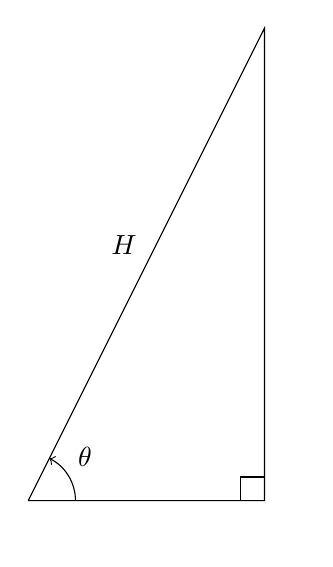
\begin{tikzpicture}
      \draw (0,0) -- node[below,transparent]{$A$} (3,0) -- %
      node[right,transparent]{$O$} (3,6) -- node[above left]{$H$} (0,0);
      \draw (3,0) -- (3,0.3) -- (2.7,0.3) -- (2.7,0) -- cycle;
      \draw[->] (0.6,0) arc (0:63.4:0.6) node[midway,above right]{$\theta$};
    \end{tikzpicture}
  }
  \only<5>{ %
    \centering
    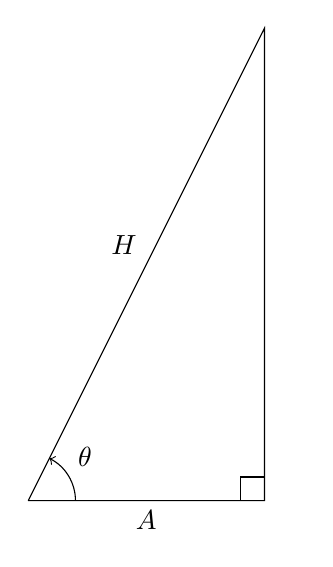
\begin{tikzpicture}
      \draw (0,0) -- node[below]{$A$} (3,0) -- %
      node[right,transparent]{$O$} (3,6) -- node[above left]{$H$} (0,0);
    \draw (3,0) -- (3,0.3) -- (2.7,0.3) -- (2.7,0) -- cycle;
    \draw[->] (0.6,0) arc (0:63.4:0.6) node[midway,above right]{$\theta$};
    \end{tikzpicture}
  }
  \only<6>{ %
    \centering
    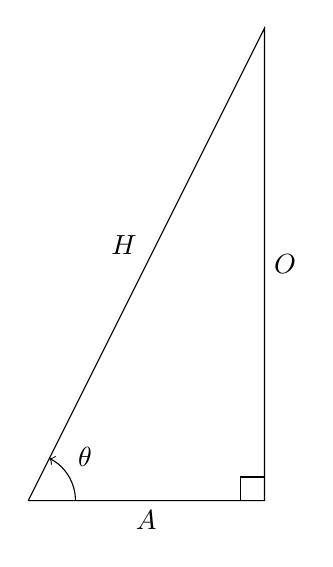
\begin{tikzpicture}
      \draw (0,0) -- node[below]{$A$} (3,0) -- %
      node[right]{$O$} (3,6) -- node[above left]{$H$} (0,0);
    \draw (3,0) -- (3,0.3) -- (2.7,0.3) -- (2.7,0) -- cycle;
    \draw[->] (0.6,0) arc (0:63.4:0.6) node[midway,above right]{$\theta$};
    \end{tikzpicture}
  }
  \end{columns}
\end{frame}

% EJD: similar triangles diagram
% EJD: show how ``tangent'' comes about ... also versine, etc.
% EJD: colours for numerator and denominator in ratios
\begin{frame}
  \frametitle{The Six Trigonometric Ratios}
  \begin{columns}
  \column{0.65\textwidth}
  \begin{itemize}[<+->]
  \item By similar triangles, the ratio between any two sides of a
    right triangle depends only on the angle, not the size of the triangle.
  \item Each of the ratios has a name.
  \item Sine ($\sin$) of the angle is O/H
  \item Cosine ($\cos$) is A/H
  \item Tangent ($\tan$) is O/A
  \item SOHCAHTOA
  \item secant ($\sec$) is H/A
  \item cosecant ($\csc$) is H/O
  \item cotangent ($\cot$) is A/O
  \end{itemize}
  \column{0.35\textwidth}
  \only<1->{ %
    \centering
    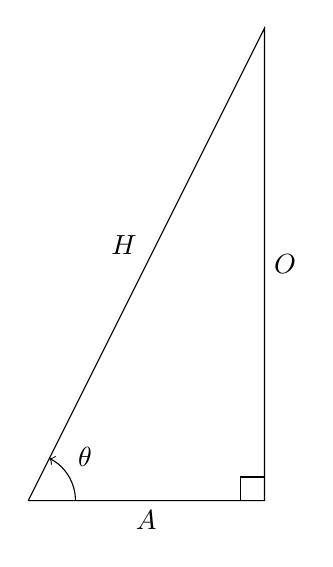
\begin{tikzpicture}
      \draw (0,0) -- node[below]{$A$} (3,0) -- %
      node[right]{$O$} (3,6) -- node[above left]{$H$} (0,0);
    \draw (3,0) -- (3,0.3) -- (2.7,0.3) -- (2.7,0) -- cycle;
    \draw[->] (0.6,0) arc (0:63.4:0.6) node[midway,above right]{$\theta$};
    \end{tikzpicture}
  }
  \end{columns}
\end{frame}

% EJD: diagram
\begin{frame}
  \frametitle{Trigonometry in Cartesian Coordinates}
  \begin{columns}
  \column{0.65\textwidth}
  \begin{itemize}[<+->]
  \item To deal with angles outside of the range $[0,\pi/2]$ we will
    find it convenient to fit our right triangle inside the unit circle.
  \item If an angle is greater than $\pi/2$ but less than $\pi$, the
    adjacent side is negative but the opposite side is still positive.
  \item In general, we have the translation adjacent $\to x$, opposite
    $\to y$, hypoteneuse $\to 1$.
  \item It follows that in quadrant I, all ratios are positive; in
    quadrant II, sine is positive but cosine and tangent are negative,
    etc.
  \item All Students Take Calculus
  \end{itemize}
  \column{0.35\textwidth}
  \only<1>{ %
    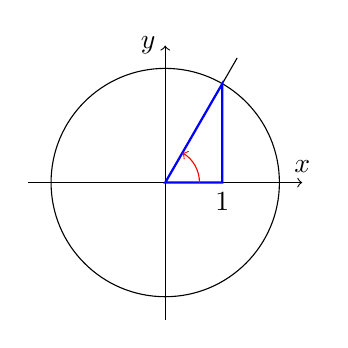
\begin{tikzpicture}[scale=0.29]
      \draw (0,0) circle (5);
      \draw[->] (-6,0) -- (0,0) -- node[midway,below]{$1$} (5,0) -- (6,0) node[above]{$x$};
      \draw[->] (0,-6) -- (0,6) node[left]{$y$};
      \draw (0,0) -- (60:6.3);
      \draw[blue,thick] (0,0) -- (60:5) -- (60:5 |- 0,0) -- cycle;
      \draw[red,->] (1.5,0) arc (0:60:1.5);
    \end{tikzpicture}
  }
  \only<2-3>{ %
    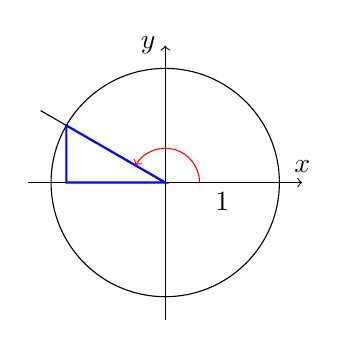
\begin{tikzpicture}[scale=0.29]
      \draw (0,0) circle (5);
      \draw[->] (-6,0) -- (0,0) -- node[midway,below]{$1$} (5,0) -- (6,0) node[above]{$x$};
      \draw[->] (0,-6) -- (0,6) node[left]{$y$};
      \draw (0,0) -- (150:6.3);
      \draw[blue,thick] (0,0) -- (150:5) -- (150:5 |- 0,0) -- cycle;
      \draw[red,->] (1.5,0) arc (0:150:1.5);
    \end{tikzpicture}
  }
  \only<4>{ %
    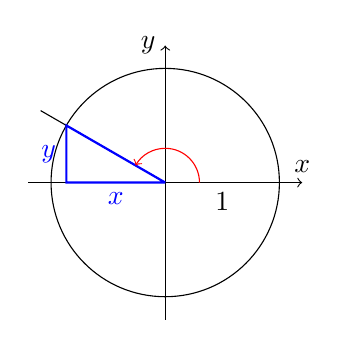
\begin{tikzpicture}[scale=0.29]
      \draw (0,0) circle (5);
      \draw[->] (-6,0) -- (0,0) -- node[midway,below]{$1$} (5,0) -- (6,0) node[above]{$x$};
      \draw[->] (0,-6) -- (0,6) node[left]{$y$};
      \draw (0,0) -- (150:6.3);
      \draw[blue,thick] (0,0) -- (150:5) -- node[midway,left]{$y$} (150:5 |- 0,0) -- node[midway,below]{$x$} (0,0);
      \draw[red,->] (1.5,0) arc (0:150:1.5);
    \end{tikzpicture}
  }
  \only<5->{ %
    \begin{tikzpicture}[scale=0.29]
      \draw[->] (-6,0) -- (6,0) node[above]{$x$};
      \draw[->] (0,-6) -- (0,6) node[left]{$y$};
      \draw node (A) at (3,3) {A};
      \draw node (S) at (-3,3) {S};
      \draw node (T) at (-3,-3) {T};
      \draw node (C) at (3,-3) {C};
    \end{tikzpicture}
    % EJD: show actual inequalities
  }
  \end{columns}
\end{frame}

\begin{frame}
  \frametitle{Exact Values for $\theta=\pi/4$}
  \begin{columns}
  \column{0.65\textwidth}
  \begin{itemize}[<+->]
  \item With a little geometry, we can work out the exact
    trigonometric ratios for $\pi/4$ radians.
  \item Inscribe a square in a circle.
  \item There are 8 identical right triangles, so the angle is
    $2\pi/8=\pi/4$ radians.
  \item By the little squares, the legs are equal.  Assume they have
    side length $1$ unit.
  \item By the Pythagorean Theorem, the hypoteneuse is
    $\sqrt{1^2+1^2}=\sqrt{2}$ units.
  \item Therefore $\sin \pi/4 = 1/\sqrt{2}$, $\cos \pi/4 =
    1/\sqrt{2}$, $\tan \pi/4 = 1/1 = 1$.
  \end{itemize}
  \column{0.35\textwidth}
  \only<2>{ %
    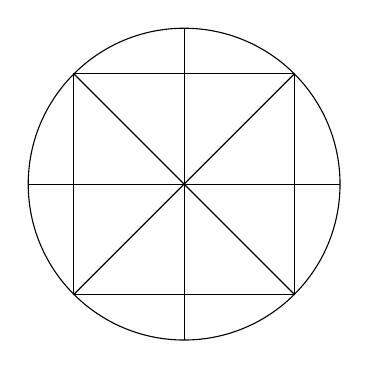
\begin{tikzpicture}[scale=1.4]
      \draw (0,0) circle ({sqrt(2)}) ;
      \draw (-1,-1)--(1,1);
      \draw (1,-1)--(-1,1);
      \draw ({-sqrt(2)},0)--({sqrt(2)},0);
      \draw (0,{-sqrt(2)})--(0,{sqrt(2)});
      \draw (1,1)--(-1,1)--(-1,-1)--(1,-1)--cycle;
    \end{tikzpicture}
  }
  \only<3>{ %
    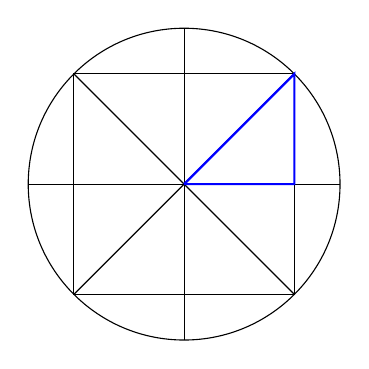
\begin{tikzpicture}[scale=1.4]
      \draw (0,0) circle ({sqrt(2)}) ;
      \draw (-1,-1)--(1,1);
      \draw (1,-1)--(-1,1);
      \draw ({-sqrt(2)},0)--({sqrt(2)},0);
      \draw (0,{-sqrt(2)})--(0,{sqrt(2)});
      \draw (1,1)--(-1,1)--(-1,-1)--(1,-1)--cycle;
      \draw[blue,thick] (0,0) -- (1,0) -- (1,1) -- (0,0);
    \end{tikzpicture}
  }
  \only<4>{ %
    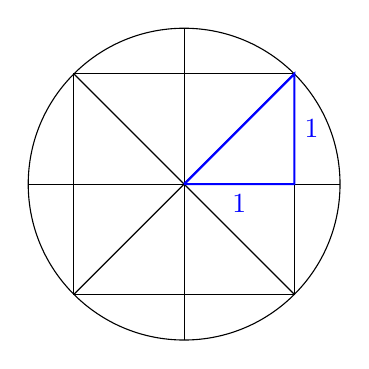
\begin{tikzpicture}[scale=1.4]
      \draw (0,0) circle ({sqrt(2)}) ;
      \draw (-1,-1)--(1,1);
      \draw (1,-1)--(-1,1);
      \draw ({-sqrt(2)},0)--({sqrt(2)},0);
      \draw (0,{-sqrt(2)})--(0,{sqrt(2)});
      \draw (1,1)--(-1,1)--(-1,-1)--(1,-1)--cycle;
      \draw[blue,thick] (0,0) -- node[below]{$1$} (1,0)-- node[right]{$1$} (1,1)-- (0,0);
    \end{tikzpicture}
  }
  \only<5->{ %
    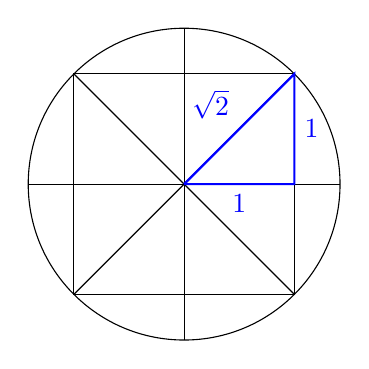
\begin{tikzpicture}[scale=1.4]
      \draw (0,0) circle ({sqrt(2)}) ;
      \draw (-1,-1)--(1,1);
      \draw (1,-1)--(-1,1);
      \draw ({-sqrt(2)},0)--({sqrt(2)},0);
      \draw (0,{-sqrt(2)})--(0,{sqrt(2)});
      \draw (1,1)--(-1,1)--(-1,-1)--(1,-1)--cycle;
      \draw[blue,thick] (0,0)-- node[below]{$1$} (1,0)-- node[right]{$1$} (1,1)-- node[above left]{$\sqrt{2}$} (0,0);
    \end{tikzpicture}
  }
  \end{columns}
\end{frame}

% EJD: draw hexagon like square above
\begin{frame}
  \frametitle{Exact Values for $\theta=\pi/3$}
  \begin{columns}
  \column{0.65\textwidth}
  \begin{itemize}[<+->]
  \item Using an equilateral triangle, we can get the ratios for $\pi/3$.
  \item Take an equilateral triangle of side $2$.
  \item All angles are $60^{\circ}=\pi/3$ rad.
  \item Drop a perpendicular from the top vertex.
  \item In the resulting right triangle, the hypoteneuse is $2$ and
    the base is $1$.  By the Pythagorean theorem the other side is
    $\sqrt{2^2-1^2}=\sqrt{3}$.
  \item It follows that $\sin \pi/3 = \sqrt{3}/2$, $\cos \pi/3 = 1/2$,
    $\tan \pi/3=\sqrt{3}/1 = \sqrt{3}$.
  \end{itemize}
  \column{0.35\textwidth}
  \only<1>{ %
    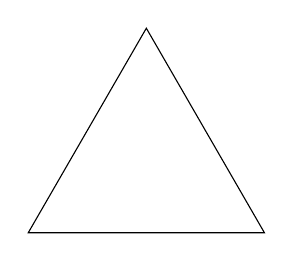
\begin{tikzpicture}[scale=0.5]
      \draw (0,0) -- (6,0) -- (60:6) -- cycle;
      %\draw[red,->] (1.5,0) arc (0:60:1.5);
    \end{tikzpicture}
  }
  \only<2>{ %
    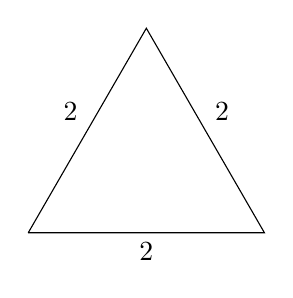
\begin{tikzpicture}[scale=0.5]
      \draw (0,0) -- node[midway,below]{$2$} (6,0) -- node[midway,above right]{$2$} (60:6) -- node[midway,above left]{$2$} (0,0);
      %\draw[red,->] (1.5,0) arc (0:60:1.5);
    \end{tikzpicture}
  }
  \only<3>{ %
    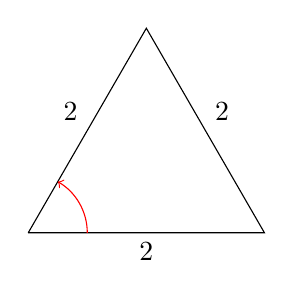
\begin{tikzpicture}[scale=0.5]
      \draw (0,0) -- node[midway,below]{$2$} (6,0) -- node[midway,above right]{$2$} (60:6) -- node[midway,above left]{$2$} (0,0);
      \draw[red,->] (1.5,0) arc (0:60:1.5);
    \end{tikzpicture}
  }
  \only<4>{ %
    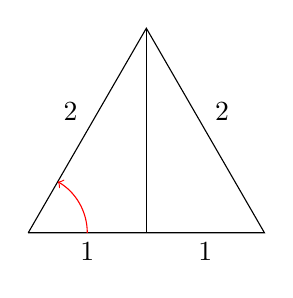
\begin{tikzpicture}[scale=0.5]
      \draw (0,0) -- node[midway,below]{$1$} (3,0) -- node[midway,below]{$1$} (6,0) -- node[midway,above right]{$2$} (60:6) -- node[midway,above left]{$2$} (0,0);
      \draw[red,->] (1.5,0) arc (0:60:1.5);
      \draw (60:6) -- (60:6 |- 0,0);
    \end{tikzpicture}
  }
  \only<5->{ %
    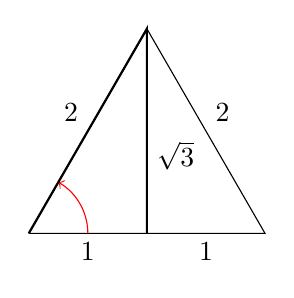
\begin{tikzpicture}[scale=0.5]
      \draw (0,0) -- node[midway,below]{$1$} (3,0) -- node[midway,below]{$1$} (6,0) -- node[midway,above right]{$2$} (60:6) -- node[midway,above left]{$2$} (0,0);
      \draw[red,->] (1.5,0) arc (0:60:1.5);
      \draw[thick] (0,0) -- (60:6) -- node[midway,below right]{$\sqrt{3}$} (60:6 |- 0,0);
    \end{tikzpicture}
  }
  \end{columns}
\end{frame}

% EJD: consider dividing the circle into 24, writing ratios in terms
% of \pi/12
% EJD: draw hexagon like square above
\begin{frame}
  \frametitle{Exact Values for $\theta=\pi/6$}
  \begin{columns}
  \column{0.65\textwidth}
  \begin{itemize}[<+->]
  \item The triangle we used is called the $1$, $2$, $\sqrt{3}$ triangle.
  \item Flipping that triangle over, we can find the ratios for
    $30^{\circ}=\pi/6$.
  \item Now the opposite side is $1$, the adjacent side is
    $\sqrt{3}$, and the hypoteneuse is $2$.
  \item The ratios are $\sin \pi/6 = 1/2$, $\cos \pi/6 = \sqrt{3}/2$,
    $\tan \pi/6 = (1/2)/(\sqrt{3}{2}) = 1/\sqrt{3}$.
  \item For all three ``special triangles'' we can also find the other
    three ratios.
  \item For example, $\sec \pi/6 = H/A = 2/\sqrt{3}$.
  \end{itemize}
  \column{0.35\textwidth}
  \only<1>{ %
    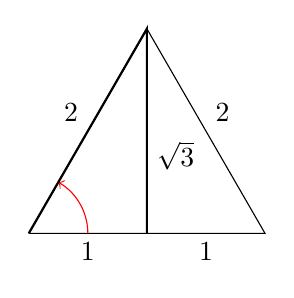
\begin{tikzpicture}[scale=0.5]
      \draw (0,0) -- node[midway,below]{$1$} (3,0) -- node[midway,below]{$1$} (6,0) -- node[midway,above right]{$2$} (60:6) -- node[midway,above left]{$2$} (0,0);
      \draw[red,->] (1.5,0) arc (0:60:1.5);
      \draw[thick] (0,0) -- (60:6) -- node[midway,below right]{$\sqrt{3}$} (60:6 |- 0,0);
    \end{tikzpicture}
  }
  \only<2->{ %
    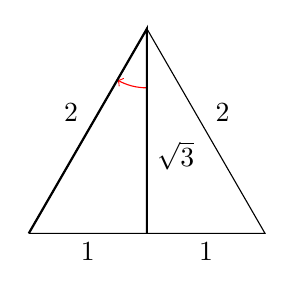
\begin{tikzpicture}[scale=0.5]
      \draw (0,0) -- node[midway,below]{$1$} (3,0) -- node[midway,below]{$1$} (6,0) -- node[midway,above right]{$2$} (60:6) -- node[midway,above left]{$2$} (0,0);
      %\draw[red,->] (1.5,0) arc (0:60:1.5);
      \draw[red,->]  (60:6) ++(0,-1.5) arc (270:240:1.5); 
      \draw[thick] (0,0) -- (60:6) -- node[midway,below right]{$\sqrt{3}$} (60:6 |- 0,0);
    \end{tikzpicture}
  }
  \end{columns}
\end{frame}

% EJD: table
% EJD: do we want to use the word ``function'' here?
\begin{frame}
  \frametitle{Table of Exact Values}
  \centering
  \begin{tabular}{|l||c|c|c|c|c|c|c|}
    \hline
    angle  & $\frac{0\pi}{12}$ &
    $\frac{1\pi}{12}$    & $\frac{2\pi}{12}$    & $\frac{3\pi}{12}$    & 
    $\frac{4\pi}{12}$    & $\frac{5\pi}{12}$    & $\frac{6\pi}{12}$    \\
    \hline
    aka    & $0$               &
    $\frac{\pi}{12}$     & $\frac{\pi}{6}$      & $\frac{\pi}{4}$      &
    $\frac{\pi}{3}$      & $\frac{5\pi}{6}$     & $\frac{\pi}{2}$      \\
    \hline
    deg    & $0^{\circ}$         &
    $15^{\circ}$           & $30^{\circ}$           & $45^{\circ}$          &
    $60^{\circ}$           & $75^{\circ}$           & $90^{\circ}$          \\
    \hline\hline
    $\sin$ & $0$               &
                         & $\frac{1}{2}$        & $\frac{1}{\sqrt{2}}$ &
    $\frac{\sqrt{3}}{2}$ &                      & $1$                  \\
    \hline
    $\cos$ & $1$               &
                         & $\frac{\sqrt{3}}{2}$ & $\frac{1}{\sqrt{2}}$ &
    $\frac{1}{2}$        &                      & $0$                  \\
    \hline
    $\tan$ & $0$               &
                         & $\frac{1}{\sqrt{3}}$ & $1$                  &
    $\sqrt{3}$           &                      & $\infty$             \\
    \hline\hline
    $\csc$ & $\infty$          &
                         & $2$                  & $\sqrt{2}$           &
    $\frac{2}{\sqrt{3}}$ &                      & $1$                  \\
    \hline
    $\sec$ & $1$               &
                         & $\frac{2}{\sqrt{3}}$ & $\sqrt{2}$           &
    $2$                  &                      & $\infty$             \\
    \hline
    $\cot$ & $\infty$          &
                         & $\sqrt{3}$           & $1$                  &
    $\frac{1}{\sqrt{3}}$ &                      & $0$                  \\
    \hline
  \end{tabular}
  \\
  \begin{itemize}
  \item Note the entries for $\csc$, $\sec$, and $\cot$ are reciprocals of the corresponding entries for $\sin$, $\cos$, $\tan$, respectively.
  \item We will fill in the missing entries when we learn about trig identities.
  \end{itemize}
\end{frame}

% EJD: show we can loop right around, >2\pi.  What about negative angles?

% EJD: diagrams.
\begin{frame}
  \frametitle{Extending Exact Values to Other Quadrants}
  \begin{columns}
  \column{0.65\textwidth}
  \begin{itemize}[<+->]
  \item Consider the angle $3\pi/4$ radians.  It lies in quadrant II.
  \item One of our special triangles appears here, but with a
    different orientation.
  \item In this case, the opposite side is $1$, but the adjacent side
    is $-1$.  The hypoteneuse is still $\sqrt{2}$.
  \item It follows that $\sin 3\pi/4 = 1/\sqrt{2}$, $\cos 3\pi/4 =
    -1/\sqrt{2}$, $\tan 3\pi/4 = 1/-1 = -1$.
  \item We can obtain similar results for all the other special
    triangles in the other quadrants.
  \end{itemize}
  \column{0.35\textwidth}
  \only<1->{ %
    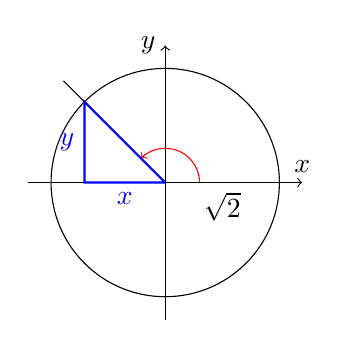
\begin{tikzpicture}[scale=0.29]
      \draw (0,0) circle (5);
      \draw[->] (-6,0) -- (0,0) -- node[midway,below]{$\sqrt{2}$} (5,0) -- (6,0) node[above]{$x$};
      \draw[->] (0,-6) -- (0,6) node[left]{$y$};
      \draw (0,0) -- (135:6.3);
      \draw[blue,thick] (0,0) -- (135:5) -- node[midway,left]{$y$} (135:5 |- 0,0) -- node[midway,below]{$x$} (0,0);
      \draw[red,->] (1.5,0) arc (0:135:1.5);
    \end{tikzpicture}
  }
  \end{columns}
\end{frame}

% EJD: graph
\begin{frame}
  \frametitle{Graph of Sine}
\end{frame}

% EJD: graph
\begin{frame}
  \frametitle{Graph of Cosine}
\end{frame}

% EJD: graph
\begin{frame}
  \frametitle{Graph of Tangent}
\end{frame}

% EJD: graph
\begin{frame}
  \frametitle{Graph of Secant}
\end{frame}

% EJD: graph
\begin{frame}
  \frametitle{Graph of Cosecant}
\end{frame}

% EJD: graph 
\begin{frame}
  \frametitle{Graph of Cotangent}
\end{frame}


\subsection{Trigonometric Identities}

% EJD: motivate identities by trying to find ratios for \pi/12?

% EJD: no diagram?
\begin{frame}
  \frametitle{Identities vs. Equations}
  %\begin{columns}
  %\column{0.65\textwidth}
  \begin{itemize}[<+->]
  \item Some equations are true only for some values of the unknown.
  \item For example, $x^2+x-2=0$ is true only for $x=-2$ and $x=1$.
  \item Other equations are true for all values of the unknown.
  \item For example, $x^2-1=(x+1)(x-1)$.
  \item We call such equations \textit{identities}.
  \item Identities give us a way to do algebra with the trig functions.
  \end{itemize}
  %\column{0.35\textwidth}
  %\end{columns}
\end{frame}

% EJD: is this the right word? co-function?
\begin{frame}
  \frametitle{Relationships among the Ratios}
  % EJD: diagrams??
  %\begin{columns}
  %\column{0.65\textwidth}
  \begin{itemize}[<+->]
  \item Our first set of identities link the various ratios.
  \item We have 
    \begin{equation*}
      \sec \theta 
      = \frac{H}{A} = \frac{1}{A/H} = \frac{1}{\cos \theta}
    \end{equation*}
  \item Similarly 
    \begin{equation*}
      \csc \theta = \frac{H}{O} = \frac{1}{O/H} = \frac{1}{\sin
        \theta}
    \end{equation*}
  \item Similarly
    \begin{equation*}
      \cot\theta = \frac{A}{O} = \frac{1}{O/A} = \frac{1}{\tan \theta} 
    \end{equation*}
  \item Finally note 
    \begin{equation*}
      \frac{\sin\theta}{\cos\theta} = \frac{O/H}{A/H} = \frac{O}{A} 
      = \tan\theta
    \end{equation*}
  \item Since they hold for any angle $\theta$, they are identities.
  \end{itemize}
  %\column{0.35\textwidth}
  %\end{columns}
\end{frame}

% EJD: diagrams
\begin{frame}
  \frametitle{The Pythagorean Identity}
  \begin{columns}
  \column{0.65\textwidth}
  \begin{itemize}[<+->]
  \item Consider our typical right triangle.
  \item Rescale by dividing through by $H$.  That does not change the
    values of the ratios.
  \item Note that by the Pythagorean Theorem, $(O/H)^2 + (A/H)^2 = (H/H)^2$
  \item Writing in terms of trig functions, $(\sin\theta)^2 +
    (\cos\theta)^2 =1$
  \item A common shorthand is to write $\sin^2 \theta + \cos^2\theta =1$
  \end{itemize}
  \column{0.35\textwidth}
  \only<1>{ % EJD: why doesn't cycle work with edge labels?
    \begin{tikzpicture}
      \draw (0,0)-- node[below,midway]{$A$} (3.5,0)-- node[right,midway]{$O$} 
      (60:7)-- node[above left,midway]{$H$} (0,0) ;
    \end{tikzpicture}
  }
  \only<2->{ % EJD: stop figure from twitching
    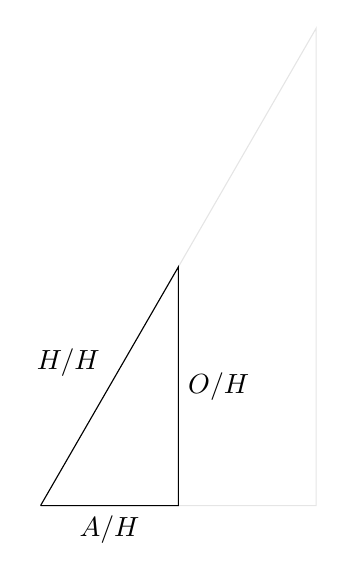
\begin{tikzpicture}
      \draw[very nearly transparent] (0,0)-- (3.5,0)--  (60:7)-- (0,0) ;
      \draw (0,0)-- node[below,midway]{$A/H$} (3.5/2,0)-- 
      node[right,midway]{$O/H$} 
      (60:3.5)-- node[above left,midway]{$H/H$} (0,0) ;
    \end{tikzpicture}
  }
  \end{columns}
\end{frame}

% EJD: diagrams
\begin{frame}
  \frametitle{Pythagorean Identity for $\tan$ and $\sec$}
  \begin{columns}
  \column{0.65\textwidth}
  \begin{itemize}[<+->]
  \item Consider our typical right triangle.
  \item Rescale by dividing through by $A$ this time.
  \item By the Pythagorean Theorem we have $(O/A)^2 + (A/A)^2 =
    (H/A)^2$
  \item In terms of trig functions, $\tan^2\theta + 1 = \sec^2\theta$
  \item Similarly, rescaling by dividing through by $O$ we have
    $(O/O)^2+(A/O)^2=(H/O)^2$
  \item In terms of trig functions,
    $1+\cot^2\theta = \csc^2\theta$
  \end{itemize}
  \column{0.35\textwidth}
  \only<1>{ % EJD: why doesn't cycle work with edge labels?
    \begin{tikzpicture}
      \draw (0,0)-- node[below,midway]{$A$} (3.5,0)-- node[right,midway]{$O$} 
      (60:7)-- node[above left,midway]{$H$} (0,0) ;
    \end{tikzpicture}
  }
  \only<2-4>{ % EJD: stop figure from twitching
    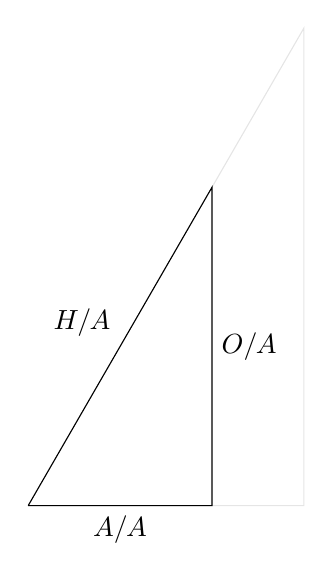
\begin{tikzpicture}
      \draw[very nearly transparent] (0,0)-- (3.5,0)--  (60:7)-- (0,0) ;
      \draw (0,0)-- node[below,midway]{$A/A$} (3.5/1.5,0)-- 
      node[right,midway]{$O/A$} 
      (60:3.5*2/1.5)-- node[above left,midway]{$H/A$} (0,0) ;
    \end{tikzpicture}
  }
  \only<5->{ % EJD: stop figure from twitching
    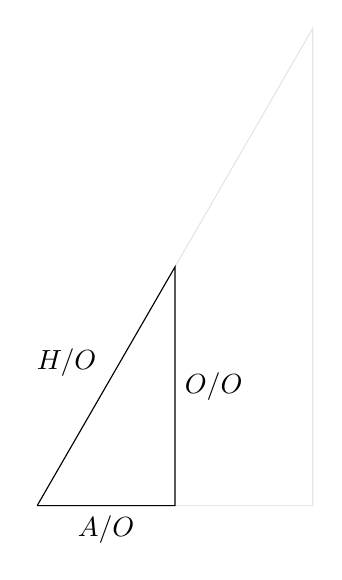
\begin{tikzpicture}
      \draw[very nearly transparent] (0,0)-- (3.5,0)--  (60:7)-- (0,0) ;
      \draw (0,0)-- node[below,midway]{$A/O$} (3.5/2,0)-- 
      node[right,midway]{$O/O$} 
      (60:3.5*2/2)-- node[above left,midway]{$H/O$} (0,0) ;
    \end{tikzpicture}
  }
  \end{columns}
\end{frame}

% EJD: show negative angle diagram
\begin{frame}
  \frametitle{Even and Odd Identities}
  \begin{columns}
  \column{0.65\textwidth}
  \begin{itemize}[<+->]
  \item Note that for a negative angle $-\theta$, 
    $O\to -O$, $A\to A$, and $H\to H$. 
  \item It follows that $\sin (-\theta) = -O/H = -(O/H) = -\sin\theta$
  \item Similarly, $\tan(-\theta)=-\tan\theta$ but
    $\cos(-\theta)=\cos\theta$
  \item We call $\sin$ and $\tan$ odd functions because of the analogy
    with odd powers: $(-x)^3 = -x^3$, $(-x)^5=-x^5$, \ldots
  \item We call $\cos$ an even function because of the analogy with
    even powers: $(-x)^2=x^2$, $(-x)^4=x^4$, \ldots
  \end{itemize}
  \column{0.35\textwidth}
  \only<1->{% 
    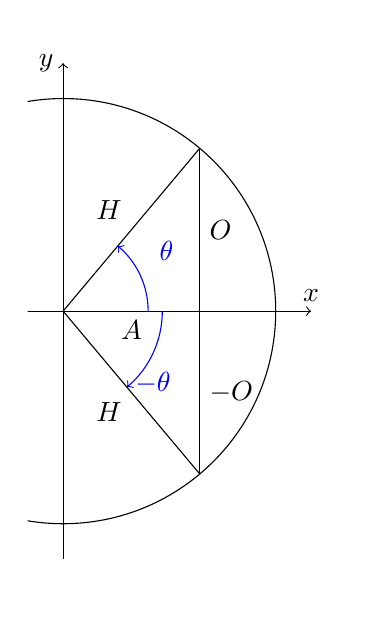
\begin{tikzpicture}[scale=0.9]
      \clip (-0.5,-4)--(4,-4)--(4,4)--(-0.5,4)--cycle;
      \draw[->] (-3.5,0)--(3.5,0) node[above]{$x$};
      \draw[->] (0,-3.5)--(0,3.5) node[left]{$y$};
      \draw (0,0) circle (3);
      \draw (0,0)-- node[above left]{$H$} (50:3);
      \draw (0,0)-- node[below left]{$H$} (-50:3);
      \draw (0,0)-- node[below]{$A$} (50:3 |- 0,0);
      \draw (-50:3)-- node[right]{$-O$} (50:3 |- 0,0) -- 
      node[right]{$O$} (50:3);
      \draw[blue,->] (1.2,0) arc (0:50:1.2) ;
      \draw node[label={[blue]25:$\theta$}] (L1) at (25:1.2) {};
      \draw[blue,->] (1.4,0) arc (0:-50:1.4);
      % EJD: move label slightly to left
      \draw node[label={[blue]270:$-\theta$}] (L2) at (-25:1.4) {};
    \end{tikzpicture}
  }
  \end{columns}
\end{frame}

% EJD: diagram of angle, angle plus 2pi
\begin{frame}
  \frametitle{Periodic Identities}
  \begin{columns}
  \column{0.68\textwidth}
  \begin{itemize}[<+->]
  \item If we go to an angle $\theta$, then go further all the way
    around the circle, we get the same final result.
  \item That means that all the trig functions should not change under
    those circumstances.
  \item So we get the identities 
    \begin{equation*}
      \sin(\theta+2\pi)=\sin\theta \quad
      \cos(\theta+2\pi)=\cos\theta 
    \end{equation*}
    \begin{equation*}
      \tan(\theta+2\pi)=\tan\theta \quad
      \cot(\theta+2\pi)=\cot\theta
    \end{equation*}
    \begin{equation*}
      \sec(\theta+2\pi)=\sec\theta \quad
      \csc(\theta+2\pi)=\csc\theta 
    \end{equation*}
  \end{itemize}
  \column{0.32\textwidth}
  % EJD: note additional slight shrinkage!! from 35% to 32%
  \end{columns}
\end{frame}

% EJD: diagram would be nice
\begin{frame}
  \frametitle{Addition Formulas for $\sin$ and $\cos$}
  %\begin{columns}
  %\column{0.65\textwidth}
  \begin{itemize}[<+->]
  \item Through some geometry that I'm not going to explain, we can
    figure out what happens when we add angles.
  \item From now on, I'm going to use $x$ and $y$ to represent two
    angles, not the adjacent and opposites sides of a triangle in a
    unit circle.
  \item For the sum of angles in the sine function, we have
    \begin{equation*}
      \sin(x+y) = \sin x \cos y + \cos x \sin y
    \end{equation*}
  \item For the sum of angles in the cosine function, we have
    \begin{equation*}
      \cos(x+y) = \cos x \cos y - \sin x \sin y
    \end{equation*}
  \end{itemize}
  %\column{0.35\textwidth}
  %\end{columns}
\end{frame}

\begin{frame}
  \frametitle{Subtraction Formulas for $\sin$ and $\cos$}
  %\begin{columns}
  %\column{0.65\textwidth}
  \begin{itemize}[<+->]
  \item Replacing $y$ with $-y$ in the addition formulas, we obtain
    the subtraction formulas.
  \item Recall the addition formula for $\sin$ is
    \begin{equation*}
      \sin(x+y) = \sin x \cos y + \cos x \sin y
    \end{equation*}
  \item Replacing $y$ with $-y$:
    \begin{equation*}
      \sin(x+(-y))=\sin x \cos(-y) + \cos x\sin(-y)
    \end{equation*}
  \item Using odd/even properties,
    \begin{equation*}
      \sin(x-y) = \sin x \cos y - \cos x \sin y
    \end{equation*}
  \item Similarly,
    \begin{equation*}
      \cos(x-y) = \cos x \cos y + \sin x \sin y
    \end{equation*}
  \end{itemize}
  %\column{0.35\textwidth}
  %\end{columns}
\end{frame}

\begin{frame}
  \frametitle{Addition and Subtraction for $\tan$}
  %\begin{columns}
  %\column{0.65\textwidth}
  \begin{itemize}[<+->]
  \item Now we can develop addition and subtraction formulas for $\tan$
  \item We have
    \begin{equation*}
      \tan(x+y)=\frac{\sin(x+y)}{\cos(x+y)}
      = \frac{\sin x\cos y+\cos x\sin y}{\cos x\cos y-\sin x\sin y}
    \end{equation*}
    % EJD: there's room for another step
  \item Dividing through by $\cos x\cos y$,
    \begin{equation*}
      \tan(x+y) = \frac{\tan x + \tan y}{1-\tan x \tan y}
    \end{equation*}
  \item Substituting $-y$ for $y$,
    \begin{equation*}
      \tan(x-y) = \frac{\tan x - \tan y}{1+\tan x \tan y}
    \end{equation*}
  \end{itemize}
  %\column{0.35\textwidth}
  %\end{columns}
\end{frame}

\begin{frame}
  \frametitle{Double Angle Formulas}
  %\begin{columns}
  %\column{0.65\textwidth}
  \begin{itemize}[<+->]
  \item Recall the angle addition formulas.
    \begin{align*}
      \sin(x+y) &= \sin x \cos y + \cos x \sin y \\
      \cos(x+y) &= \cos x \cos y - \sin x \sin y
    \end{align*}
  \item In those formulas, replace $y$ with $x$.
    \begin{align*}
      \sin(x+x) &= \sin x \cos x + \cos x \sin x \\
      \cos(x+x) &= \cos x \cos x - \sin x \sin x
    \end{align*}
  \item Doing a little algebra,
    \begin{align*}
      \sin 2x = 2\sin x \cos x \qquad
      \cos 2x = \cos^2 x - \sin^2 x
    \end{align*}
  \item Using $\sin^2 x + \cos^2x =1$ we also have
    \begin{equation*}
      \cos 2x = 1-2\sin^2x = 2\cos^2 x -1
    \end{equation*}
  \end{itemize}
  %\column{0.35\textwidth}
  %\end{columns}
\end{frame}

% EJD: save real estate by not replacing x with x/2
\begin{frame}
  \frametitle{Half Angle Formulas}
  %\begin{columns}
  %\column{0.65\textwidth}
  \begin{itemize}[<+->]
  \item Recall the double angle identities
    \begin{equation*}
      \cos 2x = 1 -2\sin^2 x \qquad \cos 2x = 2\cos^2 x -1
    \end{equation*}
  \item Replacing $x$ with $x/2$ we have
    \begin{equation*}
      \cos 2\frac{x}{2} = 1-2\sin^2 \frac{x}{2} \qquad
      \cos 2\frac{x}{2} = 2\cos^2 \frac{x}{2} - 1
    \end{equation*}
  \item Doing a little algebra we have
    \begin{equation*}
      \sin^2 \frac{x}{2} = \frac{1-\cos x}{2}
      \qquad
      \cos^2 \frac{x}{2} = \frac{1+\cos x}{2}
    \end{equation*}
  \item Taking square roots we have
    \begin{equation*}
      \left| \sin \frac{x}{2} \right| = \sqrt{\frac{1-\cos x}{2}}
      \qquad
      \left| \cos \frac{x}{2} \right| = \sqrt{\frac{1+\cos x}{2}}
    \end{equation*}
  \end{itemize}
  %\column{0.35\textwidth}
  %\end{columns}
\end{frame}

% EJD: spacing in formulas
\begin{frame}
  \frametitle{Product Formulas}
  %\begin{columns}
  %\column{0.65\textwidth}
  \begin{itemize}[<+->]
  \item Recall the angle addition and subtraction identities
    \begin{align*}
      \sin(x+y) &= \sin x \cos y - \cos x \sin y \\
      \sin(x-y) &= \sin x \cos y + \cos x \sin y
    \end{align*}
  \item Adding the two identities we get
    \begin{equation*}
      \sin (x+y) + \sin(x-y) = 2\sin x \cos y
    \end{equation*}
  \item After a slight rearrangement,
    \begin{equation*}
      % EJD: shrink 1/2
      \mbox{$\sin x \cos y = \frac{1}{2} \left( \sin(x+y) + \sin(x-y) \right)$}
    \end{equation*}
  \item By similar means
    \begin{align*}
      &\mbox{$\cos x \cos y = \frac{1}{2} \left( \cos(x+y)+ \cos(x-y) \right)$}
      \\
      &\mbox{$\sin x \sin y = \frac{1}{2} \left( \cos(x-y)-\cos(x+y) \right)$}
    \end{align*}
  \end{itemize}
  %\column{0.35\textwidth}
  %\end{columns}
\end{frame}

\end{document}

